\documentclass{thesisclass}
% Based on thesisclass.cls of Timo Rohrberg, 2009
% ----------------------------------------------------------------
% Thesis - Main document
% ----------------------------------------------------------------


%% -------------------------------
%% |  Information for PDF file   |
%% -------------------------------
\hypersetup{
 pdfauthor={Not set},
 pdftitle={Not set},
 pdfsubject={Not set},
 pdfkeywords={Not set}
}
\usepackage{booktabs} % For formal tables
\urlstyle{rm}


\usepackage{subcaption}
\captionsetup[subfigure]{list=true, font=normal, labelfont=bf, 
labelformat=brace, position=top}

\usepackage[inline]{enumitem}

\usepackage{multirow}
\usepackage[acronym,nomain,toc]{glossaries}

\usepackage{pdflscape}
\usepackage{afterpage}

\usepackage{cleveref}
\usepackage[colorinlistoftodos,prependcaption]{todonotes}
\usepackage{xargs}


\makeatletter
\def\BState{\State\hskip-\ALG@thistlm}
\patchcmd{\@verbatim}
  {\verbatim@font}
  {\verbatim@font\fontsize{11}{12}\selectfont}
  {}{}
\makeatother

% Acronyms

\makenoidxglossaries

\newacronym{DDL}{DDL}{Data Definition Language}

%% ---------------------------------
%% | Information about the thesis  |
%% ---------------------------------

\newcommand{\myname}{Simon Englert}
\newcommand{\toolAbrev}{Short Name\xspace}
\newcommand{\toolLong}{Long Name\xspace}
\newcommand{\mytitle}{Design of a Shared Parking System\\
											with special attention\\
											 to security aspects}
\newcommand{\myinstitute}{Chair for Computer Science II\\
													Software Engineering\\
													Secure Software Systems}

\newcommand{\reviewerone}{}
\newcommand{\reviewertwo}{}
\newcommand{\advisor}{Prof. Dr.-Ing. Alexandra Dmitrienko}
\newcommand{\advisortwo}{}

\newcommand{\timestart}{22. June. 2018}
\newcommand{\timeend}{30. August. 2018}
\newcommand{\submissiontime}{30. August. 2018}

%% ---------------------------------
%% | ToDo Marker - only for draft! |
%% ---------------------------------
% Remove this section for final version!
\setlength{\marginparwidth}{20mm}

\newcommand{\margtodo}
{\marginpar{\textbf{\textcolor{red}{ToDo}}}{}}

\newcommandx{\toDo}[2][1=]{\todo[linecolor=green,inline,backgroundcolor=green!25,bordercolor=green,#1]{\textbf{ToDo: }#2}}

%% --------------------------------
%% | Settings for word separation |
%% --------------------------------
% Help for separation:
% In german package the following hints are additionally available:
% "- = Additional separation
% "| = Suppress ligation and possible separation (e.g. Schaf"|fell)
% "~ = Hyphenation without separation (e.g. bergauf und "~ab)
% "= = Hyphenation with separation before and after
% "" = Separation without a hyphenation (e.g. und/""oder)

% Describe separation hints here:
\hyphenation{
% Pro-to-koll-in-stan-zen
}


%% ------------------------
%% |    Including files   |
%% ------------------------
% Only files listed here will be included!
% Userful command for partially translating the document (for bug-fixing e.g.)



\includeonly{%
titlepage,
declaration,
00_abstract,
00_abstractgerman,
01_introduction,
02_related_work_and_background,
03_system_model_and_requirements,
04_design,
05_security_analysis,
06_implementation,
07_future_work,
08_conclusion,
09_acknowledgements,
appendix
}


%%%%%%%%%%%%%%%%%%%%%%%%%%%%%%%%%
%% Here, main documents begins %%
%%%%%%%%%%%%%%%%%%%%%%%%%%%%%%%%%
\begin{document}
\begin{large}
% Remove the following line for German text
\selectlanguage{english}

\frontmatter
\pagenumbering{roman}
%% titlepage.tex
%%

% coordinates for the bg shape on the titlepage
\newcommand{\diameter}{20}
\newcommand{\xone}{-15}
\newcommand{\xtwo}{160}
\newcommand{\yone}{15}
\newcommand{\ytwo}{-253}

\begin{titlepage}
% bg shape
\begin{tikzpicture}[overlay]
\draw[color=gray]  
 		 (\xone mm, \yone mm)
  -- (\xtwo mm + \diameter pt , \yone mm)
  -- (\xtwo mm + \diameter pt , \ytwo mm) 
	-- (\xone mm , \ytwo mm)
	-- (\xone mm, \yone mm);
\end{tikzpicture}
	\begin{textblock}{10}[0,0](4,2.5)
		
\includegraphics[width=.3\textwidth]{logos/unilogo4cohne_mittel.jpg}
	\end{textblock}
	\changefont{phv}{m}{n}	% helvetica	
	\vspace*{3cm}
	\begin{center}
		\Huge{\mytitle}
		\vspace*{2cm}\\
		\Large{
			\iflanguage{english}{Bachelor Thesis of}			
												  {Masterarbeit\\von}
		}\\
		\vspace*{1cm}
		\huge{\myname}\\
		\vspace*{1cm}
		\Large{
			\iflanguage{english}{At the Department of Computer Science}			
													{Am Institut f\"ur Informatik}
			\\
			\myinstitute
		}
    
	\end{center}
	\vspace*{.2cm}
	\begin{center}
	
\includegraphics[width=.3\textwidth]{logos/seal.eps}
	\end{center}
\Large{
\begin{center}
\vspace{.5cm}
\begin{tabular}[ht]{l c l}
  % Gutachter sind die Professoren, die die Arbeit bewerten. 
  %\iflanguage{english}{Reviewer}{Gutachter}: & \hfill  & \reviewerone\\
  %\iflanguage{english}{Second reviewer}{Zweitgutachter}: & \hfill  & \reviewertwo\\
  \iflanguage{english}{Advisor}{Betreuender Mitarbeiter}: & \hfill  & \advisor\\
  %\iflanguage{english}{Second advisor}{Zweiter betreuender Mitarbeiter}: & \hfill  & \advisortwo\\
  % Der zweite betreuende Mitarbeiter kann weggelassen werden. 
\end{tabular}
\end{center}
}


%\vspace{2cm}
%\begin{center}
%\large{\iflanguage{english}{Duration}{Bearbeitungszeit}: \timestart \hspace*{0.25cm} -- %\hspace*{0.25cm} \timeend}
%\end{center}


\begin{textblock}{10}[0,0](3.2,16.75)
\small{ 
	\iflanguage{english}
		{Julius-Maximilians-Universit\"at W\"urzburg}
		{Julius-Maximilians-University, W\"urzburg}
}
\end{textblock}

\begin{textblock}{10}[0,0](13.2,16.75)
\large{
	\textbf{www.uni-wuerzburg.de} 
}
\end{textblock}

\end{titlepage}

\cleardoublepage
\vspace*{36\baselineskip}
\hbox to \textwidth{\hrulefill}
\par
\iflanguage{english}{I declare that I have developed and written the enclosed thesis completely by myself, and have not used sources or means without declaration in the text.}{Ich versichere wahrheitsgem\"a\ss, die Arbeit selbstst\"andig angefertigt, alle benutzten Hilfsmittel vollst\"andig und genau angegeben und alles kenntlich gemacht zu haben, was aus Arbeiten anderer unver\"andert oder mit Ab\"anderungen entnommen wurde.}

\textbf{Wuerzburg, 30.08.2018}
\vspace{1.5cm}

\dotfill\hspace*{8.0cm}\\
\hspace*{2cm}(\textbf{\myname}) %center name with hspace

\thispagestyle{empty}
\blankpage

%% -------------------
%% |   Directories   |
%% -------------------
\tableofcontents
\clearpage
\blankpage



\blankpage

\section*{Abstract}
As major cities are growing more and more, the parking situation in those cities is becoming more precarious than ever. Parking demand already exceeds the limited amount of parking spaces available, and thus people searching for a place to park generate a significant part of those cities traffic. This leads to frustration with drivers, more traffic jams, unnecessary use of petrol and further air pollution. The creation of new parking spaces is often either difficult or very expansive, which means existing parking spots have to be used more efficiently. Solutions realizing that idea to try and solve those problems are for the most part called intelligent parking systems. This thesis is focused on Shared Parking, a special kind of intelligent parking system, which opens the possibility of sharing a parking place between different people. This work features the design and implementation of such a system with special attention given to security aspects.


\blankpage
\section*{Abstract (Deutsch)}
Mit dem zunehmenden Wachstum der Großstädte wird die Parksituation in diesen Städten prekärer denn je. Die Nachfrage nach Parkplätzen übersteigt bereits die begrenzte Anzahl an Parkplätzen, so dass Menschen, die auf der Suche nach einem Parkplatz sind, einen erheblichen Teil des Verkehrsaufkommens dieser Städte generieren. Dies führt zu Frustration bei den Fahrern, mehr Staus, unnötigem Benzinverbrauch und erhöhter Luftverschmutzung. Die Schaffung neuer Parkplätze ist in der Regel schwierig oder sehr kostspielig, so dass vorhandene Parkplätze effizienter genutzt werden müssen. Lösungen, die diese Idee verwirklichen, um die genannten Probleme zu lösen, werden meist als intelligente Parksysteme bezeichnet. Diese Arbeit beschäftigt sich mit Shared Parking, einer speziellen Art von intelligentem Parksystem, das die Möglichkeit eröffnet, einen Parkplatz zwischen verschiedenen Personen zu teilen. Diese Arbeit beinhaltet die Konzeption und Implementierung eines solchen Systems unter besonderer Berücksichtigung von Sicherheitsaspekten.


%% -----------------
%% |   Main part   |
%% -----------------
\mainmatter
\pagenumbering{arabic}
\chapter{Introduction}
\label{ch:Introduction}
Parking in large cities is a well-known problem. For decades, the search for a parking space has been something that annoys most people. Due to the ever faster growing cities in recent years, the resulting difficulties are only intensifying. The ensuing traffic for example already represents a significant part of the total traffic in city centres. According to studies around 30 percent of the daily city traffic comes from car park seekers\cite{shoup2006cruising}. In addition to the rising number of people in cities, the percentage of people who own a car continues to increase, which adds to the traffic problems. However, the traffic is not just frustrating for the drivers. The ensuing traffic jams and the slow-moving traffic cause an increased amount of petrol to be burned and the air to become additionally polluted. Especially in these times, when air pollution and climate warming are becoming even more important due to Dieselgate and the capricious weather conditions, one should be looking for a solution.

The creation of new parking spaces is rarely an option. On one hand, this is often associated with high costs, on the other hand, there is usually no space for the construction of new parking spaces available in the cities. Instead, existing parking spaces must be used more effectively.

This can be done in many different ways. So-called intelligent parking systems increase the smartness of parking in different areas and therefore often lead to a more effective use of parking spaces. Intelligent parking systems are available in various forms and there are numerous scientific papers and completed projects for most of them. However, there are hardly any relevant developments for shared parking systems, which are by definition a type of intelligent parking system. A shared parking system is a trading platform on which private users can rent out and rent parking spaces. Sharing systems, such as car sharing, have become increasingly influential in recent years and are expected to continue to grow strongly \cite{freese2014shared}. If an object is shared among different users, it is used more effectively. This applies to parking places and a shared parking system as well. Therefore, the main part of this work will be concerned with designing a shared parking system. Special attention is paid to security aspects by detailing how the system handles fraud.

First, an overview of the system is presented, in particular the system model, which depicts the different roles in our shared parking system. This is followed by functional and security requirements to be met by the design. In contrast to existing systems, the design of our system will try avoid complex hardware and manual intervention by the service provider. In addition, this work deals in particular with fraud in a shared parking system and ways to deal with it. Possible cases of fraud within the system are described and grouped into different classes of fraud. It is noted that our system must be able to recognize and prevent all of them, punish adversaries and compensate injured parties.

The actual design is described in the next step. First all functional features and then the security features that determine how to deal with fraud are explained. We will introduces various modules that help dealing with fraud. There is a rating module, a module for reporting adversaries, a module to help verify fraud cases and a reputation module, which assigns a score to each user that indicates how trustworthy that user is.

Subsequently, the design is evaluated on the basis of the requirements. We shall find, that our system is robust against all the attacks listed before. The shared parking system therefore complies with the specified security requirements and can successfully deal with all classes of fraud cases.

Once it has been shown that the design meets the requirements, an implementation of a prototype, which is also part of this study, will be discussed in more detail. The design was implemented as a client-server model and includes a Java web service, which serves as an interface to a central database, and an Android app for the end user. All three parts are described in detail and it is explained how to execute the attached code and get the prototype up and running. At the end of the chapter, some aspects, which could be applied to help with the realization of this shared parking system, are pointed out.

Finally, a number of future work topics are presented which were not processed in this study. In the future, for example, alternative reputation systems could be applied and evaluated or the performance and good usability of the app could be proven.

At the end, a summary of the achieved results is provided.
\chapter{Related Work and Background}
\label{ch:Related Work and Background}
If one takes a look at existing work in the field of intelligent parking systems, he will encounter countless scientific papers in the most diverse sub-areas of intelligent parking systems. In addition, there are numerous projects in which such systems have already been implemented. There are also some works that have set themselves the task of categorizing related work in this field. Nevertheless, there does not seem to be any definite consensus among scientists on definitions and categorizations. In the following we will present an introduction to the topic based on these papers.

\section{Overview}

\subparagraph{Intelligent Parking Systems}
In general terms, intelligent parking systems, also called smart parking systems, are systems that try to solve the countless parking problems mentioned in \ref{ch:Introduction} while integrating 'advanced technologies and researches from various academic disciplines' \cite{idris2009car}. Thus the words intelligent or smart have different meanings depending on the time at which a system was developed \cite{fraifer2016investigation}. With further progress, especially in computer science, new opportunities are opening up and old implementations no longer seem to be 'advanced' or 'smart', but were at the time of development.
\subparagraph{Shared Parking}
Shared Parking Systems form a separate category of intelligent parking systems, because they use the emerging 'shared technology' in connection with mobile devices, which are available to most people due to technological advances and cheaper prices. Shared parking provides the framework for making purely private parking spaces available to the public by allowing them to be traded as a commodity. \cite{itdp2014shared} By sharing, parking spaces can be used more effectively and parking information can be distributed more easily, which reduces the aforementioned parking problems. It is taken advantage of the fact that most private parking spaces are only used by certain groups of motorists at particular times and thus remain unused for a large part of the time, and that those parking times for the different groups often do not overlap\cite{vtpi2015shared}. A supermarket, for example, needs its parking spaces mainly during the day when the supermarket is opened, while a hotel needs the parking spaces at night for the overnight guests.\\
\section{Intelligent Parking Systems}
To give an overview for intelligent parking systems we are introducing a categorization of those systems proposed by Susan Shaheen in \textit{Smart parking management field test: A bay area rapid transit (bart) district parking demonstration} \cite{shaheen2005smart}. Shaheen divides intelligent parking systems into five categories.
\subparagraph{Guidance Information Systems}
Guidance information systems are the simplest type of intelligent parking systems. The aim of such systems is to point the car park seeker to the nearest available parking spaces. In many cities this is done by simple displays on the streets, which point to car parks and show the number of free parking spaces available in real time.

\subparagraph{Transit-Based Information Systems}
Transit-based information systems are just like the previously mentioned GIS pure information systems. However, special importance is given in this case to draw attention to and to direct to parking spaces that are linked directly to local public transport. In most cases such parking spaces are called 'Park+Ride' and allow free parking, for example. The main objective of these systems, in addition to reducing the traffic of those seeking parking, is to prevent any traffic in the city centers. The aim is to make public transport more attractive and usable in order to prevent air pollution and congestion in the cities themselves. 

\subparagraph{Smart Payment Systems}
With smart payment systems service providers try to minimize their maintenance costs. Setting up, emptying and repairing coin-operated machines at parking lots is often an expensive business. Operators of Smart Payment Systems therefore try to forgo using these machines. Instead, the customer pays, even contactless, with smartcards or via his own smartphone. This usually has advantages for both sides. For the customer the payment process is accelerated and he can avoid using cash and at the same time the operating costs are reduced for the service provider.

\subparagraph{E-parking}
By e-parking, Shaheen referred to a special system that was under development in 2005 by a research consortium. The aim of the concept was to combine the various smart parking ideas. The system includes advanced guidance information systems, smart payments methods, reservation options and connectivity to other digital services. More generally, we consider e-parking to be systems that use all means of digitalisation to make the parking experience better and more effective for the user in all possible aspects. Our shared parking system will take over many of the features of e-parking.

\subparagraph{Automated Parking}
Automatic parking is a system in which the user simply drives the car to a general drop-off point and later picks it up from there. The system takes over the remaining transport route of the vehicle from the delivery point to the actual parking lot. Such systems also exist as manual versions, then called valet parking.

\section{Shared Parking}
Shaheen, like many others, pays little to or no attention to the topic of shared parking. However, according to the above definition, shared parking is a kind of intelligent parking system. Overall, there are hardly any scientific papers on this subject. There are already a few implementations of the idea, but these are either limited to certain cities or have hardly any users, which renders them useless. In addition, these systems are operated by private companies and therefore no information about the security within the system is publicly available.\\

Of the few scientific papers that exist, most are concerned with the allocation and pricing of parking spaces to potential tenants.

Shao et al. \cite{shao2016simple} and Yu et al. \cite{yu2018optimal} propose to use integer linear programming to maximize profits. Both studies show that their proposed strategies, in contrast to 'first-come-first-serve' or 'first-book-first-serve' strategies, lead to higher parking space utilisation and greater profits for operators of shared parking systems. Yu et. al. refer in their work only to the sharing of parking spaces of shopping malls at night. This also implies that, unlike our system, there is no fluctuation in the number of parking spaces over time which their system would not be able to handle.

Xu et al. \cite{xu2016private} extend a classic matching mechanism (Top Trading Cycles, ttc) for the parking spaces to allow cash flow. They assume that each participant owns at least one parking space and participates with this parking space in the ttc mechanism. For situations where participants are unable to rent out their own parking space or do not wish to rent another parking space, the mechanisms (Price-compatible) Top Trading Cycles and Deals (TTCD)' and 'Price-compatible Top Trading Cycles and Chains (PC-TTCC)' are proposed as extensions to ttc. These allow, in addition to the already possible exchange of parking spaces in ttc, the flow and exchange of money within the system. These mechanisms allowe participants to save costs, but under certain circumstances negative platform's payoff would occur. 

Xiao et al. \cite{xiao2018shared} assign parking spaces to tenants using a double auction mechanism. They present the Demander Competition Padding Method (DC-PM) auction mechanism based on a slot allocation rule and a transaction payment rule. Both demanders and bidders place their bids by specifying the parking price and time and the mechanism determines the allocation of the parking spaces. Since this mechanism can lead to distorted social welfare, a Modified Demander Competition Padding Method (MDC-PM) auction mechanism is proposed as well, which is however inferior to the first mechanism in terms of its usefulness for the participants. They show that both mechanism "can realize asymptotic efficiency as both demanders and suppliers approach infinity", but do not take the spatial requirements of the participants into account during the allocation process. 

Zhang et al. \cite{zhang2019pricing} try to improve the competitiveness of shared parking lot providers compared to traditional parking lots. They use the Hotteling model to compare the product differentiation of the two parking systems and use equilibrium analyses to evaluate the parking prices. 

In all these papers, the utilisation of parking spaces or the social welfare in the system improves compared to the 'first-book-first-serve' mechanism, but the systems do not provide the user with the same level of transparency. In our shared parking system, users should be able to see exactly which parking spaces are available, choose from them and be sure to be able to use the selected parking space. This can only be implemented with 'first-book-first-serve' and the systems mentioned above are not able to provide this functionality.\\

In addition to parking space allocation through a matching mechanism, Kim et al. \cite{Kim2015ASP} propose an infrastructure to help drivers find the optimal parking space. The infrastructure consists of Road Side Units (RSUs), which communicate with the cars of parking seekers and Fog servers, which monitor the availability of each parking lot. RSUs communicate directly with Fog servers in their vicinity and with each other through a Roadside Cloud. Users can make parking requests while driving, which are then accepted by the RSUs. Through communication between the RSUs and the Fog Servers, a matching problem with all car park seekers is established, solved and the allocation of parking spaces is sent back to the vehicles through the RSUs. 

The big problem for this system are the expensive implementation and maintenance costs which arise because a lot of hardware and sensors have to be installed. The operator has to provide the RSUs, the Fog Server, sensors for each parking spot and the Roadside Cloud. Every participant requires appropriate channels of communication on his car to connect to the RSUs. Our system, on the other hand, will do without expensive hardware to reduce maintenance costs, thus enabling nearly anyone to participate.\\


A number of shared parking platforms have already been implemented, but in very few cases they have become established. Internationally, for example, justpark.com or mobypark.com offer this service, in Germany there are providers like parkplace.de and parklist.de. All these platforms offer private individuals the opportunity to offer their own parking spaces, but in most cases the supply of parking places is very limited.

At parkinglist.de, even in large German cities such as Munich, there is almost exclusively only information about public car parks or offers for monthly rented parking spaces from car park operators, but there are hardly any private offers.

At parkplace.de there is also only a small number of almost exclusively long-term parking spaces available. Moreover, this platform does not offer the possibility to automatically perform payments. Instead, payment-specific matters have to be agreed on with the landlord separately.

At justpark.com, which originates from England, there are, for example in London, almost exclusively public parking garages available. However, many car parks also offer the possibility of making reservations.

At mobypark.com you can find some listings from private persons. However, Mobypark is not widespread and is only really represented in a few cities, such as Amsterdam and Paris.

However, none of these service providers discloses information on how they can protect their systems and users from fraud and how they generally deal with adversaries. This is presumably because, as Mobypark itself reports on its website, parking spaces are hardly rented for short periods of time like a few hours, but mainly for longer periods (several days to several months). In addition, most of the rented parking spaces are not publicly accessible and key cards or the like must be exchanged prior to and at the end of the rental process. These conditions already lead to a reduction of fraud possibilities. In our application, however, it should also be possible to rent freely accessible parking spaces, even for short periods of time. This creates new opportunities for fraud, which, unlike in the scientific papers mentioned above, we will address in this paper.

\section{Trust Systems}\label{sec:Trust Systems}
In order to distinguish malicious and genuine users in our system, we will use a trust system. Since there is a large amount of scientific work and discussion in the area of trust systems, we will not develop any new methods ourselves and will instead fall back on already matured methods, adapt them to our system and thereby make them better fit.\\

Trust systems are used in many different forms for many different purposes. Therefore, we have sought to find methods developed for systems that are similar to ours. Finally, we will use a trust method from the area of Mobile Participatory Sensing Applications. These are systems in which participants use smartphones or similar devices to send information that they received at various locations through the sensors of their devices to a backend server. We will later show how trust methods of such systems can easily be mapped to our trust system. Mousa et. al. wrote a survey on this topic in 2015, which gives a fundamental overview of this area of trust systems\cite{mousa2015trust}:\\

In all these systems, trust is used to assess the reputation of individual users. The calculated reputation is therefore a value for the trustworthiness of the participants and the quality of their contributions. Mousa classifies trust/reputations systems according to methodology, type of distribution and anonymity of participants. 

\subparagraph{Methodology} Either a Trusted Platform Module (TPM) or a reputation score can be used as a methodology for trust assessment. TPMs are hardware chips that are installed in the devices of the participants and are therefore not suitable for our system. In the section \ref{ch:Future Work}, trust assessment using TPMs is discussed briefly. For our system, however, the use of a reputation score, which is calculated directly from the behavior of the participant, is suitable. For the computation of this score the participants' latest activities and his old score are used.

\subparagraph{Type of distribution} The distribution in a trust system can be either central, collaborative or a combination of both. Since our trust score should be hidden from the participants and we possess a trust server, a centralized structure is suitable for us. In this case the trust server receives all information, i.e. the contributions and feedback of the participants, from which it is able to calculate the score of all participants. In collaborative systems, however, each participant computes a separate score for all other participants.

\subparagraph{Anonymity of participants} Finally, anonymous and non anonymous systems can be distinguished. In anonymous systems the anonymity of the participants is preserved. This is neither necessary nor useful in our system, as each participant must provide certain personal data to access our system. \\

In the section \ref{sec:Reputation Module} reputation module we will use a trust system corresponding to the above established classification and modify it for our purposes.

The use of such a trust system however allows different types of attacks which are described in more detail in section \ref{sec:Adversary Model and Assumptions} adversary model. In \ref{ch:Security Analysis} security analysis we will finally show the robustness of our system against these attacks.

\chapter{System Model and Requirements}
\label{ch:System Model and Requirements}
Now that an overview of the topic has been provided, the next part will deal with a basic system model and the requirements that will be imposed on the design. The system model gives an overview of the different parties that exist in our shared parking model and their relationships with each other. The subsequent requirement analysis is divided into functional and security requirements. Special attention is paid to ensuring that the design is secure. For us security requirements do not only refer to standard security aspects such as encryption, user authentication and authentification, but in particular to the goal of designing our shared parking system in a way that it has the ability to handle fraud independently. For instance, the system should prevent and punish individual users from scamming other users or the system. Various forms and examples of such fraud will be considered and evaluated. The system design presented in Chapter \ref{chapter:Design} will adhere to these requirements. We will now start of with a high-level overview of the shared parking system.

\section{High-level Overview}\label{High-level Overview}
This section gives a high-level overview of the proposed shared parking system and deals with the basic capabilities of the system. The shared parking system adheres to the definition supplied at the beginning. It offers a platform for an online marketplace where both private and business users can rent and lease parking spaces. End users have the opportunity to install an app and participate in the marketplace using their smartphone. This also clarifies the basic capabilities of the system. Every user can offer his own parking spaces for specified periods of time on the platform for rent. Users can also view other users' listings, choose from them and rent those parking spaces. In this system, particular importance is given to handling fraud. The subsequent requirements define the exact framework under which the design was developed. Unlike state-of-the-art shared parking systems, our system will largely do without expensive hardware, which leads to high deployment costs for service providers and users in other systems. In addition, the system should operate mostly without manual intervention by the service provider, thus keeping maintenance costs low. Another unique feature of our system is that it can handle different attacks and fraud. No other shared parking system published, has, to our best knowledge, the ability to deal with all the different cases of fraud we define later on. In contrast to many other access control systems, our system does not aim at preventing unauthorized access of adversaries to parking spaces, but instead incorporates mechanisms to punish misbehaving users. Enforcing access control to parking lots would likely require installation of special equipment on parking lots, which we ruled out above because it would increase deployment costs of the system and raise entrance limits for landlords, which is undesirable. These mechanisms include, for example, a rating module that allows users to rate each other after each rental operation. Also part of those mechanisms is a reporting module that allows users to report adversaries. In addition, there is a module that verifies the validity of reported fraud cases through the service of other users. Finally, there is a module that monitors all processes within the system and calculates a reputation score for every user based on those. This score reflects the trustworthiness of a user.

\section{System Model}\label{System Model}
The following system model, which is depicted in figure xy, shows the various parties in our \textbf{shared parking system} $SPS$. On the one hand, there is exactly one \textbf{operator} or \textbf{service provider} $SP$. The $SP$ is responsible for the implementation of the design, operating the $SPS$ and making the systems services available to the users. The \textbf{users} $U$ are those who utilize the $SPS$. They can be divided into two roles, whereby a user can be part of both roles at different points in time. On the one hand, there are \textbf{landlords} who own a private \textbf{parking space} and want to rent it out over a certain period of time. On the other hand, there are \textbf{tenants} who are looking for a free parking space to rent for a specific time period.

This work covers fraud in $SPS$ in detail. In the \textbf{case of fraud}, users take on new roles. On the one hand there is the \textbf{adversary}, who is committing fraud, on the other hand there usually is an \textbf{injured party}, which has a disadvantage caused by the fraud case.

As mentioned in \ref{High-level Overview} we will utilize different modules that deal with those fraud cases. In each of those modules users once again assume different roles.

The rating module deals with \textbf{ratings}. For each rating there is one user who issues, called the\textbf{ rating user} and one user who receives, called the \textbf{rated user}.

The reporting module deals with \textbf{reports}. One report belongs to one case of fraud. For each report there is one user who issues, called the \textbf{reporting user} and one user who receives, called the \textbf{reported user}.

The verification module verifies reports and the corresponding fraud case. Users who verify the reports are called \textbf{inspectors}.

In the reputation module, \textbf{contributions} from all \textbf{participants} of one fraud case are processed. The participants include the reporting user, reported user and the inspectors. A participants' contribution is the information he provides about the fraud case.

All roles are described in more depth in the detailed description of the modules.\\

To-Do: Figure of system model

\section{Functional Requirements}
The following will cover the main functional requirements in detail.
\subparagraph{Low deployment cost and of the shelf hardware} Neither the operator nor the user should need any additional and expensive hardware. For getting the system to work the user just needs a off-the-shelf smartphone and the operator only needs to provide enough computational power to get the server running. There will be no sensors installed at the parking spots, no additional hardware used for confirming parking time or the likes of that.
\subparagraph{Automatic Processing} Where possible, the $SPS$ should be prevented from requiring manual intervention by the $SP$. The system should be able to run all basic use cases should and may only request manual intervention in exceptional cases. On the one hand this should lead to a fast processing of all inquiries and on the other hand reduce the costs for the $SP$ stemming from employing people for manual tasks.
\subparagraph{Streichen: Neutral Balance} The operator or the system has different costs and revenues. Thus, the operator can either make a profit or lose money. We impose the condition on the system that in the long run, the revenues at least cover or even exceed the costs. This means that there may be time spans in which the costs are greater than the revenues, but if you take a look at the system in the long term, the revenues must surpass the costs.

\subparagraph{More to come}hi\\

There are also areas that do not place any functional requirements. There are aspects to which no special significance is attached in this work. This includes, for example, all legal matters. On the one hand, this work is in the field of computer science and the author does not have the fundamental knowledge to evaluate and judge legal matters. On the other hand, the legal aspect of a shared parking system involves many and various legal factors, which would exceed the scope of this work. Nevertheless, attention was paid during the design to carry out as little legal interference as possible in order to avoid legal difficulties during the implementation.

\section{Adversary Model and Assumptions}

\section{Adversary Model and Classes of Fraud}
When we talk about fraud, we mean a user's ability to scam other users or the system using its normal functionality in order to gain a profit. In many cases, this has a negative impact on other users. There are numerous possibilities for fraud in the system, some of which are mentioned as follows. We will categorize all fraud cases into three different classes. As mentioned in \ref{System Model} we refer to a user who commits fraud as a adversary. Users who are affected by fraud in a negative way will be called injured or injured party. \\

\subparagraph{Class 1} The first class of fraud cases are the result of the general nature of a shared parking system. This class consists of fraud cases where a tenant has booked a parking space, but it is not available when he arrives. There could be different possibilities as to why the parking space is not available, examples of which are the following.
\begin{itemize}
\item adversary parks in a car park, which another user has booked for this time.
\item Tenant overstays his booked parking time.
\item Landlord rents out a parking space, but remains on it himself.
\item Landlord offers the same parking space multiple times.
\item Landlord offers a parking space that does not exist.
\end{itemize}
To deal with these class 1 cases, we will introduce various modules, such as a report module and a reputation module, which enables detection of the attacks described above. As we will see later, Class 1 cases can be handled by our system without manual intervention. 

\subparagraph{Class 2} The reputation module helps to deal with class 1 cases of fraud, however it itself is subject to a new series of fraud cases. We group these new fraud cases into class 2. All well known attacks in this area are described in \cite{mousa2015trust} and are applied to our system as follows:
\begin{itemize}
\item \textbf{Corruption attack:} An adversary unintentionally or deliberately sends corrupted data and information. An example of a corruption attack is when a reporting user enters an incorrect license plate number for the reported user.
\item \textbf{On-off attack:} An attacker alternates between malicious and genuine behavior. This is particularly difficult to detect when the transition appears to occur randomly.
\item \textbf{Re-entry attack:} An adversary tries to white wash his trust value by rejoining the system with a new identity. In our system this corresponds to a new registration of an existing user.
\item \textbf{Collusion:} Several adversaries act together and execute attacks collectively. Joint attacks have a greater impact on the system and are harder to detect than acting independently.
\item \textbf{Sybil attack:} This is an extension of the re-entry attack. An adversary creates multiple identities or accounts within the system and utilizes them in a collusion attack.
\item \textbf{Reputation lag exploitation:} The adversary uses the period between his first attack and the evaluation and corresponding downgrading of his trust value to launch a large number of attacks.
\item \textbf{GPS spoofing attacks:} The adversary tampers with the GPS location of his device.
\item \textbf{Unfair ratings:} The adversary does not rate another user according to his genuine opinion.
\item \textbf{Bad mouthing or negative discrimination attack:} The adversary raises false accusations or assigns a bad rating to a genuine user.
\item \textbf{Ballot stuffing or positive discrimination attack:} The adversary does not report misbehaviour or assigns a good rating to a malicious user.
%User tries to impose costs on to the system by doing false reports. adversary pretends to be the injured party. adversary accuses another user of fraud.
\end{itemize}
We shall see that Class 2 cases can also be dealt with mostly without manual intervention by using a robust reputation module. 

\subparagraph{Class 3} While the first two classes cover the main and most frequent cases of fraud, there are others. Class 3 cases differ from the other classes in that it will not be possible to solve them without manual intervention. These are exceptional cases that occur only in low frequency. Examples are given below.
\begin{itemize}
\item Landlord rents out parking spaces that they do not own themselves.
\item Tenant cancels booking of a parking space without paying.
\end{itemize}
For this class of fraud cases, we will also show methods of dealing with them.\\

Most of these attacks can only be performed by registered users. In contrast, however, there is a case of fraud, which can also be carried out by persons outside the system. A parking offender who occupies a booked, private parking space does not necessarily have to be registered in the system. Dealing with this problem is not the main focus of this work, but a suggestion on how to deal with it when realizing the system will be provided in section \ref{...}.

\section{Assumptions}
In the following we specify assumptions that apply to our system.\\

\subparagraph{Attacker collaboration} We assume that adversaries can not only attack the system on their own, but collaborate with other adversaries to jointly start and carry out attacks. We will show that even under this assumption the $SPS$ can protect itself from  the attacks described above.

\subparagraph{Sufficient parking spaces} We assume that there are always enough parking spaces available for compensation. The assumption is reasonable, since if the system has low occupancy levels, a suitable free parking space can always be found. If this is not the case, there will always be landlords  who offer their parking spaces for a particularly expensive and overpriced costs. These places will still be vacant even in situations where almost all capacities are occupied. These are parking spaces that are still available for use as compensation for injured parties, even when there is a high level of occupancy. 

\subparagraph{Majority assumption} We assume that the majority of users in our system are acting according to the rules, meaning that there are always a maximum of 50 percent adversaries. Even under the \textit{attacker collaboration} assumption it is reasonable to believe that there will be plenty of genuine users that use the system for parking and not for fraud as this is a typical assumption for distributed systems (e.g. \cite{benenson2004secure}, \cite{nojoumian2014efficient}, \cite{avoine2005gracefully}). One can expect that the majority of people are genuine, especially when they know that offenses are being punished hard. We further offer an opportunity to report inadvertent misdemeanors, in order to prevent major penalties, by yourself, which should prevent inadvertent misdemeanors by genuine users.\\

\section{Security Requirements}
The following will cover the main security requirements in detail. On the one hand, requirements are made on information security and on the other hand, requirements are mode on how to deal with fraud in the shared parking system. \\

The system must be able to handle all these cases of fraud mentioned in the adversary model above successfully. In the following we will define what we mean by 'successful handling'. We therefore set requirements that must be met for the various cases of fraud.
\subparagraph{Fraud Prevention} The design of the system should be such that fraud is fundamentally prevented. If this is not possible in all cases, it should be ensured that it is not worth the effort for the adversary or that adversaries are quickly discovered. This is where the second point comes into play.
\subparagraph{Fraud Detection} The system should be able to detect fraud. This includes, on the one hand, the simple recognition of fraud and, on the other hand, the ability to correctly identify the adversary. The later is particularly important for the next point.
\subparagraph{Fraud Punishment} The design should be such that a adversary can be punished by the system. After a adversary is detected, the system should always be able to penalize him. Punishment can also support the first requirement by acting as a deterrent for fraud.
\subparagraph{Fraud Compensation} Finally, the system should be able to compensate an injured party. If injured are compensated, there is no need for genuine users to worry about fraud and thus enhances the attractiveness of the system.\\

There are also areas that do not place any special requirements on security. Even without a shared parking system, attacks on the private parking infrastructure are possible. One person can for example park their car in another person's private car park. The injured party has two options, both of which can have strong disadvantages for him. He could call the towing service, hope that the adversary has not left by its arriving time or he will have to bear the expensive towing fees himself. The other option is to do nothing and look for a new parking space for yourself. Such problems, which are already present, do not need to be solved. However, it can be seen as a added bonus to prevent such problems with good design choices for the shared parking system.
\chapter{Design}
\label{ch:Design}
With the requirements being defined, the next part is devoted to the actual design. As with the requirements, we will first have a look at the functional features before dealing with fraud.

\section{Functional features}
The functional features will be presented as use cases.
\subparagraph{User registration} The registration process is rather simple. A user registers by entering his e-mail address, his first and last name and a password. After confirming the data, a mail is sent to the specified address, in which the user must verify whether it actually is his address.

\subparagraph{User login} After registering a user can log into the system at any time using his mail address and password. A user will be kept logged into the app to use all other features described below until he chooses to log out.

\subparagraph{Balance system} Each user has a credit balance that can be charged and paid out using standard payment options. Various events, such as renting or hiring out a parking space, lead to an increase or decrease to the credit balance. The precise calculation of the credit is defined below for the individual events. If a user's balance is negative, they will no longer be able to use the system. His credit must be recharged before his next action.

\subparagraph{Parking Space management} Before a user can rent out a parking space, he has to register it with the system. For parking place registration users enter the address and location (latitude and longitude) of the parking place, which then will be stored in the system. In addition to registration, these parking spaces can also be edited and removed.

\subparagraph{Renting out a parking space} If a user wants to rent out a parking space, he creates an offer. He selects one of his parking spaces, specifies the time at which the parking space is available and the price per hour. Parking offers can also be edited and removed.

\subparagraph{Car management} Before a user can book a parking space, he has to register his car with the system. For car registration he just enters the license plate. It is possible to register many cars, but a user has to choose one active car, that he can change from time to time and that gets used when he is renting a parking space. Cars can also be removed.

\subparagraph{Renting a parking space} If a user wants to rent a parking space, first a map is presented. There his location can be displayed or he can search for a city/address to be centered. All currently available parking spaces are displayed on this map. In addition to the location, the user can specify the time at which he wishes to book the parking space. If he does, only parking spaces that are available for the entire time period are displayed.

\subparagraph{Contracts Management} Users are able to look through their past, present and future parking contracts both as tenant and landlord.
  
\section{Security features}
The security features are introduced to prevent fraud and are represented by different modules. There is a rating module, reporting module and a verification module, all of which are explained below. These modules work together and provide information for a reputation module that assesses the trustworthiness of each user. At the end of this section an example is given on how the design utilizes those systems to handle fraud.

In the following descriptions of the modules a few parameters are required which are not yet specified in this work. To assign fixed numbers to these parameters, the $SPS$ should first be run through simulations or tried with test groups. Since this was not part of this study, however, we have not yet assigned fixed figures to these parameters.

\subsection{Rating Module} The design of the $SPS$ includes a rating module, allowing users to rate each other. After each rental agreement has been concluded, both tenant and landlord have the opportunity to give the other party a rating. The rating consists on the one hand of a points/star rating between 1 and 5, and on the other hand of a rating text. The user should share his experiences made with the other party and evaluate how satisfying the agreement went for him. The ratings each user received are displayed on his user page and in all of his offers. The rating system is designed to help eliminate adversaries and encourage users to be as friendly and courteous as possible.

\subsection{Reporting Module} The next important component is the reporting module. Whenever a user detects a rule violation by another user, he has the possibility to report it. For each report a distinction is made between the reporting user, the reported user and the inspectors, who will be explained in the section \ref{sec:Verification Module} later on.

First, there is the possibility of reporting a violation that occurs during a rental contract. This means another user and not the tenant who booked the parking place blocks it (fraud class 1). On the overview page of the contract, a tenant can choose to report this. He just has to enter the license plate of the adversary. It can also be reported using this function, if a booked parking space does not exist at all. Second, there is the possibility of reporting a violation that occurs not during a rental contract. This is the case when an adversary, who is unauthorized to, parks in a users parking space. This kind of report can be issued on the overview page of a parking spot. The reporting user also has to enter the license plate of the adversary. Finally, there is the possibility to report something that does not fit into the other two categories. In addition, all three report functions are combined on one report overview page in the app.

If the system receives a report, it can be sure that it is always a case of fraud. Either the user reports a real fraud case, which then has to be fraud class 1, or it is a false report from an adversary, which he expects to benefit from. This would again be a case of fraud, which can be classified in fraud class 2. The system must therefore first check the truth of a report. The verification module exists for this purpose and is explained below. After the verification module has identified who the adversary is, the necessary steps for punishment can be taken. The section \ref{section:Sanctioning and Compensation} \nameref{section:Sanctioning and Compensation} explains in detail how exactly the system acts to compensate or punish users.

\subsection{Verification Module}\label{sec:Verification Module} Another important security tool is the verification module. It allows the system to check who has really committed a rule violation. If a rule violation situation occurs and another user cannot occupy his legally entitled parking space, he will report it to the system. Since the report may also be false, the system must first verify who the real offender is: the reported user or the reporting user. For this purpose, other users are called upon to head to this place and to make a contribution to this case. Those users will then be called inspectors. The truth of the report can be verified by comparing the contributions of the reported user, the reporting user and the inspectors. The inspectors will receive a bonus on their balance for their service.

The module works in several steps. After a report is received, potential inspectors are selected and requested. They confirm whether they will verify the event or not. Afterwards, they verify the event and the system evaluates the contributions. \\

Since the location of the inspectors must be taken into account when selecting them, users have the option of deciding whether they want to participate in the verification system or not. There are two ways for all participating users to provide the system with location information. 
\begin{itemize}
\item The user allows the app to retrieve GPS data from the mobile device. The GPS data is only collected if a report needs to be verified. Directly after viewing the data, it is calculated whether the user is in the area, and the GPS data is deleted again.
\item The user selects an area on a map in which he generally agrees to verify reports in. GPS data is not necessary in this case.
\end{itemize}

First, a list of all users that are eligible for verification to a case is created. This means only users who have agreed to participate in the verification system and who are either in the vicinity of the location of the event themselves or whose verifying area contains the location of the event are chosen. This list will now be sorted in a way that the users who are most suitable are at the top and users who are less suitable are at the bottom. Suitability is determined using a connection score $con$, which is calculated for all available inspectors. This score indicates the independence between the inspector and the reporting and the reported user. A low score is a sign of great independence. $con$ represents the number of common events between the inspector and the reporting user plus the number of common events between the inspector and the reported user in a certain period of time (e.g. the last six months). The following events increment the score between user $u_1$ and $u_2$ by a single point:
\begin{itemize}
\item $u_1$ books a parking space from $u_2$.
\item $u_1$ reports $u_2$.
\item $u_1$ verifies a report from $u_2$.
\end{itemize}

Next, the users from the list are asked whether they are able and willing to verify this event. This request is not sent to all users at the same time. Based on the reputations score it is determined how many inspectors n are needed to solve the case and requests are sent to the first n*3 inspectors of the list. The lower the reputation score of a user, the more inspectors get requested for his case.\\

The selected users will receive a notification on their smartphone indicating the location of the event for review. They then confirm or reject whether they are able and willing to perform the verification within the next 30 minutes. If a user refuses or does not respond within 15 minutes, he will be removed from the list and the next user not yet contacted will receive a request. After n users have accepted the request, all other requests are revoked.\\

As soon as a user has accepted the request, he will receive exact information about the parking space. He then moves to the location of the event and states whether this parking space exists and which car is parked on it according to the license plate.\\

In the last step the contributions must be evaluated. This is done using the reputation system described below. For this purpose, the reputation of both parties to the conflict is assessed. As seen down below, not the trust values of the two parties are compared, but the trust of the contributions by those parties, in which both the trust value and other parameters have an influence. These other parameters include, for example, the inspectors' contributions and the ratings the two parties have received. \\

The verification module returns the user whose contribution possesses the lower trust value as the adversary. \\

In addition to the above, the verification module asks the reported user for feedback on this case. The reported user can either confirm or contradict the report of the reporting user. This is intended as a means of self-reporting by the reported user, which can reduce his punishment and does not negatively affect his reputation score. This is a good way for a genuine user to admit inadvertent misconduct. If a reported user confirms the accusation by the reporting user, no more inspectors need to be requested and the verification module returns the reported user as the adversary. However, even if the reported user admits the fraud with his contribution, the case is passed to the reputation module to update the reputation scores of the participating users.

\subsection{Reputation Module}\label{sec:Reputation Module} The last part of the security features is the reputation module. It stores a reputation score $R_u$ for each user $u$, which is updated using the other security modules and saved in the central database, hidden from the users. The value indicates the trustworthiness of a user. It is needed to decide who is right in the event of a conflict. Based on this reputation score, a separate trust value $Trust(C)$ is determined for each contribution $C$ taking other parameters into account. In all cases where the contributions of the reporting and the reported user do not match, this value is used to decide which contribution is considered as the truth. \\

Our reputation module is instantiated on the Dynamic Trusted Set Based Reputation System (DTSRS) developed by Mousa et. al. \cite{mousa2017reputation}. It utilizes state-of-the-art trust systems presented in \cite{mousa2015trust} and offers better evaluation results than those. DTSRS was created for use in Mobile Participatory Sensing Applications, but is also suitable for our purposes. It utilizes an ever-changing trusted set of participants to calculate the ground truth and compares all contributions to this ground truth value. In the calculation of its trust score it further takes ratings and a proximity score into account. In the following we will explain the system, our changes to it and the mapping of our parameters to those of the DTSRS. \\

The reputation module uses a trust score to evaluate participants and their contributions. The trust of a contribution $Trust(C)$ is the probability that contribution $C$ is correct. The reputation score $R_u$ of a user $u$ is the synthesized probability that his contributions are and will be correct. In $SPS$, every user can be a participant of any fraud case, but the number of particpants changes from case to case. After all, the participants in each case are the reported user, the reporting user and all inspectors. Each participant of a case submits exactly one contribution for this case. The contributions are therefore the report by the reporting user, the confirmation or denial of the report by the reported user and the verification contributions from the inspectors.\\

After every report received by the system, $R_p$ of all participants $p$ involved in the report is updated. In addition, the trust of the contributions of the reported user and the reporting user is evaluated. The trust is updated in these five steps:

\subparagraph{Contribution Evaluation}In the first step, the contributions $C_p$ by participants $p$ are evaluated and a contribution evaluation value $\theta_p $ is calculated. In our case, the contributions are the report by the reporting user, the confirmation or denial of the report by the reported user and the contributions from the inspectors resulting in $n$ contributions. In the original DTSRS, the values of the contributions are within a certain range. For our module we assume the special case that each of these contributions has exactly one of two values: (0) the contribution is consistent with the contribution of the reporting user or (1) the contribution is not consistent with the contribution of the reporting user. The two values occupy exactly the margins of the original range. This allows us to continue calculating in exactly the same way as DTSRS.

DTSRS first arranges ${C_1, ..., C_n}$ in descending order based on corresponding reputation scores ${R_1, ..., R_n}$. The first $m<n$ contributions of that order form the trusted set. The mean $\mu(C)$ of those $m$ contributions of the trusted set is then regarded as the ground truth. The module then calculates the contribution deviation $d_p$ for every contribution as depicted in the equation below and normalizes it to range [0,1].  If $d_p^{no}$, which represents the normalized value, equals 0 it is implied that $C_p$ equals the ground truth. A normalized deviation of 1 implies a complete contradiction to the ground truth. With the help of an exponential distribution and $d_p^{no}$, a score between 0.37 and 1 is assigned, which corresponds to the contribution evaluation value $\theta_p $ of the contribution $C_p$.\\

\begin{equation}
  \mu(C)= \frac{\sum_{i=1}^{m} C_i}{m}
\end{equation}
\begin{equation}
  d_p = abs(C_p - \mu(C))
\end{equation}
\begin{equation}
  d_p^{no} = \frac{d_p-\min_{i=1}^{n}(d_i)}{\max_{i=1}^{n}(d_i) - \min_{i=1}^{n}(d_i)}
\end{equation}
\begin{equation}
  \theta_p = exp^{-d_p^no}
\end{equation}

\subparagraph{Feedback Processing}In this step, the feedback each participating user received is taken into account. The module calculates a aggregated feedback score $\alpha_p$ for each participating user $p$. In DTSRS, the user can receive feedback for each contribution. There, feedback refers to exactly one contribution and is then discarded. In $SPS$, users receive feedback through the rating module. Thus, received ratings originate not only from participant, but from all users of the shared parking system. In order to avoid using a rating more than once in the calculation of a user's reputation score, \textit{feedback processing} utilizes exactly those ratings that have been entered since the user's reputation score was last updated. For the calculations, the ratings $F_r(p)$ (1 to 5 stars) of a participant $p$ given by rating user $r$ are normalized to the range [0,1]. Only ratings of users $r$ whose reputation score is greater than that of the rated participant $p$ are used ($R_r>R_p$). The individual ratings are weighted according to the reputation score of the rating user and the average is calculated, which also falls within the range [0,1]. The following equations describe the calculation, where $F$ is the number of rating users for each participant and $FH$ the number of rating users whose reputation score is higher than the reputation score of the rated user.
\begin{equation}
  F_{r,Eval}(p)=F_r(p)*R_q\; \forall r \in 1,2,...F, where\; R_r>R_p 
\end{equation}
\begin{equation}
  \alpha_p = \frac{\sum_{r=1}^{r=FH}F_{r,Eval}(p)}{FH}
\end{equation}

\subparagraph{A Temporal Proximity Factor} In DTSRS, the proximity factor measures the distance between the participant and the sensing area, as a larger distance is more likely to result in inaccurate measurements. In $SPS$, the distance has no influence on the measurements, as anyone making a contribution must be at the location of the event. Instead, however, the temporal distance $\beta_p$ has an effect on the measurements, because the more time passes, the greater the probability that the situation at the location of the event will change, which results in inaccurate measurements. For this reason, we are dealing with a temporal proximity factor $\sigma_p$ in the range [0,1], which is calculated using an inverse Gompertz function from the temporal distance. For the reported and reporting user the temporal distance is 0 and the proximity factor is therefore maximum at 1. For every other participant $\beta_p$ describes the distance between the report and the participant's contribution in minutes.
\begin{equation}
  \sigma_p = 1 - a * e^{-be^{-c\beta_p}}
\end{equation}

\subparagraph{Trust Mapping} The trust of a contribution $Trust(C)$ is calculated exactly as with DTSRS. We take a weighting $\sum_{i_1}^{4} W_i = 1$, the three already calculated values contribution evaluation $\theta_p$, aggregated feedback $\alpha_p$ and the temporal proximity factor $\sigma_p$ and as a fourth value the reputation score $R_p$ of the participant $p$ and calculate the weighted average of these four values:
\begin{equation}
  Trust(C) = W_1 * \theta_p +W_2 *  \alpha_p +W_3 *  \sigma_p +W_4 *  R_p
\end{equation}
The reputation score of a new participant is first set to 0, meaning he or she must first earn the trust of the system.

\subparagraph{Reputation Update} When updating the reputations value of a participant $p$, DTSRS only uses the contribution evaluation $\theta_p$ and not the complete trust $Trust(C)$ of his contribution. The reason for not using the proximity factor $\sigma_p$ is, that it cannot be influenced by the user and does not depend on the genuineness of the user. The temporal proximity factor is also not included in the recalculation of the reputation score in our module, as users further away from the location of the event take more time to reach the location, regardless of whether they are malicious or genuine.

The new reputation value $R\prime\prime$, as we can see in a moment, will be calculated on the basis of the old reputation value $R_p$. Because of that we dont use $Trust(C)$ for the calculation, as $R_p$ would therefore have two times the impact. Mousa et. al. also argue that with the omission of $R_p$ recent behaviour has a direct influence on the reputation score.

However, they do not provide any reason why agregated feedback $\alpha_p$ should not be included in the reputation update. Since the feedback in our system is independent of the individual contributions, but clearly provides a indication about the trustworthiness of a user, we will include it.\\

We update the reputation value consecutively with the contributions evaluation $\theta_p$  and the aggregated feedback $\alpha_p$. For both values there is a threshold $\tau_\theta$ and $\tau_\alpha$. If the previously calculated values $\theta_p$ or $\alpha_p$ of a participant $p$ is higher than $\tau_\theta$ or $\tau_\alpha$, the reputation value is increased by $e_{+,\theta}$ or $e_{+,\alpha}$. If it is lower, the reputation value is decreased by $e_{-,\theta}$ or $e_{-,\alpha}$. $e_{-,\theta}>e_{+,\theta}$ and $e_{-,\alpha}>e_{+,\alpha}$ applies to punish adversaries more severely. The update is described by the following equations: 
\begin{equation}
  R\prime_p = \begin{cases} R_p + e_{+,\theta}\quad if\; \theta_p>=\tau_\theta \\ R_p - e_{-,\theta}\quad if\; \theta_p<\tau_\theta \end{cases}
\end{equation}
\begin{equation}
  R\prime\prime_p = \begin{cases} R\prime + e_{+,\alpha}\quad if\; \alpha>=\tau_\alpha \\ R\prime - e_{-,\alpha}\quad if\; \alpha<\tau_\alpha \end{cases}
\end{equation}

If the value is above 1 or below 0 after the update, it is reset to the corresponding value (1 or 0).

\subsection{Sanctioning and Compensation}\label{section:Sanctioning and Compensation} With these basic systems it is now possible for the system to punish adversaries and compensate the injured parties. 

After a report has been received, the reporting user will first be provided with a new parking space, regardless of whether it later turns out that he was in fact the fraudster. For this purpose, the system selects the nearest parking space available for the entire duration of the reservation of the original parking space. The system now books this parking space for the reporting user, takes over the costs, and sends the information about it to his smartphone. The System however, will not pay the price which is officially offered for the replacement parking space, but will instead pay the average price of parking spaces in the area. This is calculated as the average price of all bookings of the last x months in a maximum distance of y kilometers. On registration, all users agree to make their parking space available as a replacement parking space for the average parking fee, if required. The reporting user can now use the replacement parking space and the owner of the replacement parking space will be fairly remunerated.

After a replacement parking space has been provided, the already explained verification and reputation modules are used to determine who the adversary is.

After the real offender is identified, he will be punished. The punishment of fraudsters is primarily enforced by a fine. The penalty will be deducted from his credit balance. This penalty will also be used to cover the costs of the fraud. Costs arise on the one hand when compensating the injured party and on the other hand when paying the inspectors. The penalty is calculated from the sum of the inspectors' credit bonuses and the remuneration of the landlord of the replacement car park. Thus there are no costs for the system when the offender is successfully identified.

\subsection{Example}
Figure \ref{img:example-grafik} on page \pageref{img:example-grafik} shows fraud within the system and how to deal with it. The procedure is explained in more detail below.\\

User $u_1$ bookes a parking space that belongs to user $u_2$ in advance. The $SPS$ transfers the parking fee from $u_1$ to $u_2$, while deducting the system fee and providing it to $SP$. However, when $u_1$ arrives to occupy the parking space, he realizes that another user ($u_3$) is blocking the parking place. $u_1$ then uses the reporting system to report $u_3$ with his license plate. The system receives the report and then assigns other independent users with the task of verifying the report. $u_{i1}$...$u_{i3}$ are the first to accept the verification request and head to the location of the event. In the meantime, $u_1$ will be provided with a new parking space (parking space of $u_4$). He can park on it free of charge for the same time period he booked parking spot of $u_2$. The $SP$ will cover the parking fee $f_p$ for now and add it to the balance of $u_4$. After arriving at the location of the event, $u_{i1}$...$u_{i3}$ confirm the license plate of $u_3$ and thus the report made by $u_1$. They get paid with the verification fee $f_v$ by the $SP$. The reputation module evaluates all contributions, which leads to deciding $u_3$ as the adversary. The reputation scores $R_{u_1}, R_{u_2}, R_{u_{i1}}, R_{u_{i2}}, R_{u_{i3}}$ are updated, leading to a score decrease for $u_3$ and an increase for the other users. In the end the $SPS$ deducts the fine from the balance of $u_3$ which is the sum of $f_p$ and $f_v * 3$. Thus paying for the inspectors service and the replacement parking space for $u_1$. \\

\begin{figure}
	\centering
	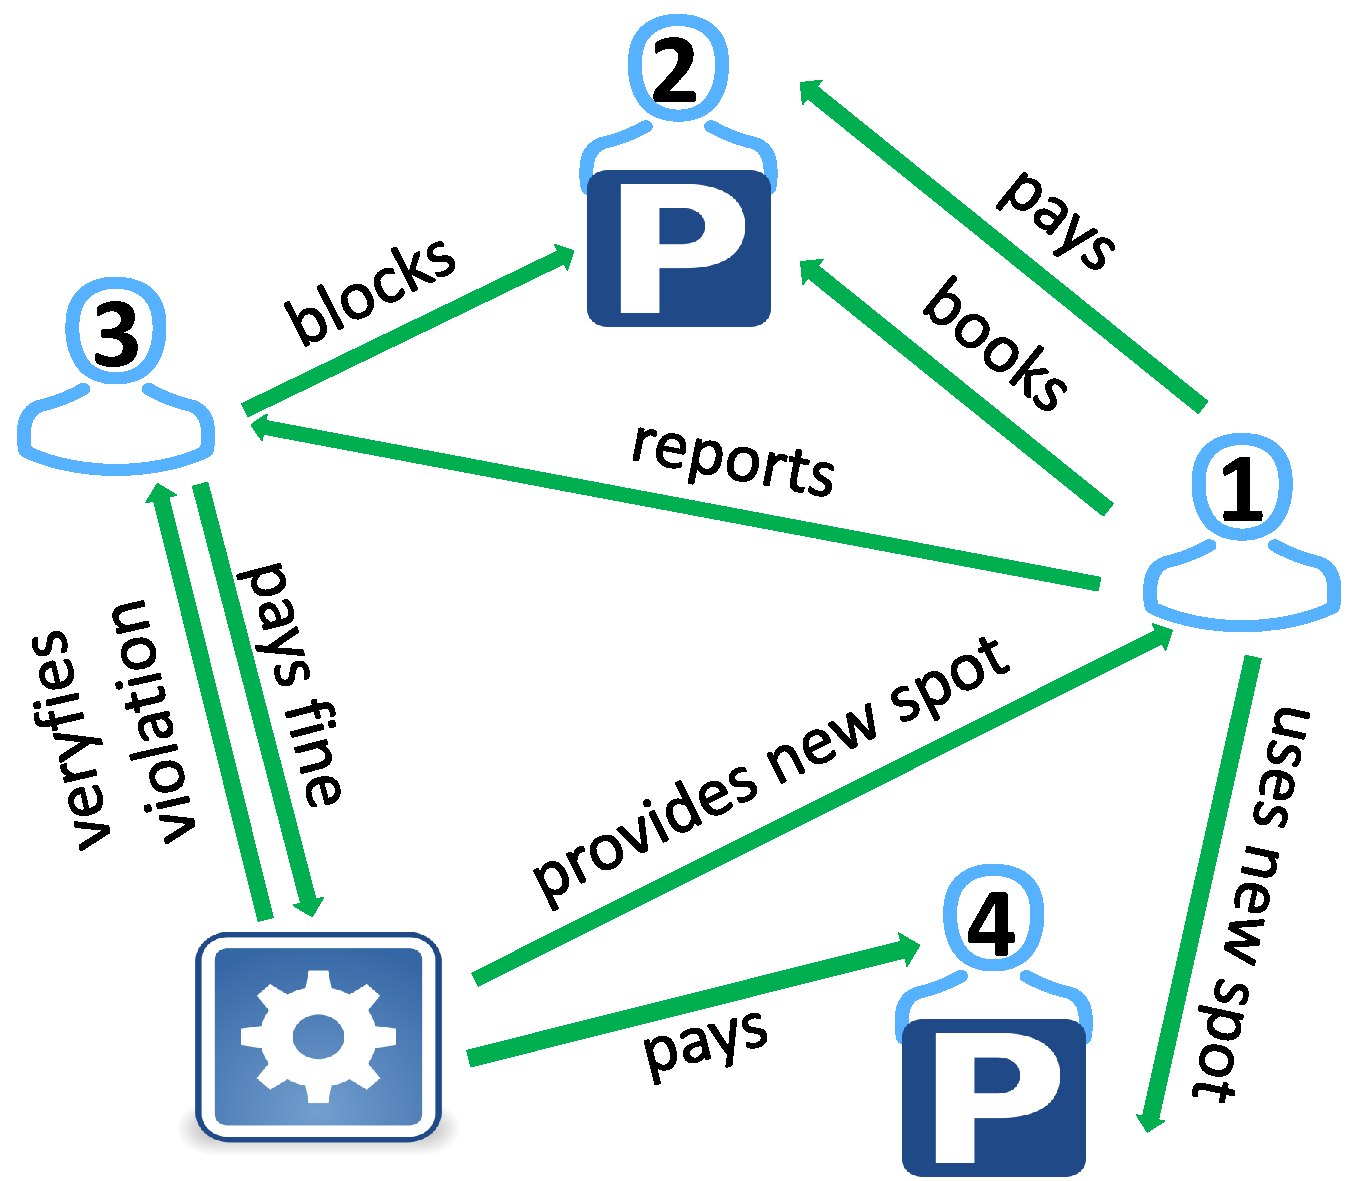
\includegraphics[width=13cm,height=11cm]{logos/example-grafik.pdf}
	\caption{A possible example for the handling of fraud}
	\label{img:example-grafik}
\end{figure}
 
The case we have just discussed is clearly a class 1 fraud case, but it might also be as follows: $u_1$ arrives at the location of the booked parking space of $u_2$ and finds a free parking space. He, however, wants to harm $u_3$ and reports him nonetheless as a parking offender. This represents a corruption attack by $u_1$ and thus a fraud case of class 2. Like above the inspectors $u_{i1}$...$u_{i3}$ are requested, except this time they'll report that the parking lot is available. The reputation module evaluates all contributions and concludes that $u_1$ is the adversary. All reputation scores $R_{u_1}, R_{u_2}, R_{u_{i1}}, R_{u_{i2}}, R_{u_{i3}}$ are adjusted accordingly.\\

We can consider another variation of the first case presented. $u_3$, who has already been exposed as adversary several times, occupies the parking lot of $u_2$ without permission and is reported by $u_1$. After the inspector $u_{i1}$ has arrived and reported his contribution, $u_3$ leaves the parking space and the other two inspectors $u_{i2}$,$u_{i3}$ report that the parking space is free. The reputation module evaluates the contributions here as well. Only two of the five contributions ($C_{u_{1}}$ and $C_{u_{i1}}$) agree with the reporting user and therefore the truth, but the module would nevertheless count them as the truth expose $u_3$ as the adversary. This is because the trust of the two contributions $Trust(C_{u_{1}})$ and $Trust(C_{u_{i1}})$ that match the reporting user is significantly higher than the trust of the other three contributions $Trust(C_{u_{i2}})$,$Trust(C_{u_{i3}})$ and $Trust(C_{u_{3}})$. The reason for this is that the proximity factors $\sigma_{u_{i2}}$ and $\sigma_{u_{i3}}$ are lowered, because $u_{i2}$ and $u_{i3}$ arrived late at the location of the event and the reputation score $R_{u_3}$ is already low, because $u_3$ is a known adversary. Thus the module returns $u_3$ as the adversary.
\chapter{Security Analysis}
\label{ch:Security Analysis}
In the following, the design of the system is evaluated using the security features set up in the requirement analysis. We look at each point individually and use the premises set up in section x to prove that we meet the requirements. To show that the reputations module is resistant to the attacks mentioned in section x, we will use the evaluation of DTSRS presented in \cite{mousa2017reputation}.

\section{Fraud Detection}
Fraud detection includes two components: the simple recognition of the fact of fraud as well as the ability to correctly identify the adversary.  \\

\subparagraph{Fraud recognition} Fraud recognition is exclusively achieved by the report system. As soon as a user detects a rule violation, he can report it and the system is informed. It is sufficient to recognize fraud by which another party would be harmed, because this would not be any different without the Shared Parking System. A parking offence only causes problems if another user, who is authorized to park, wants to park on it and with our system the other user now has the ability to report it. Thus, parking spaces with a shared parking system always provide a better possibility for fraud detection than without it. \\

\subparagraph{Adversary identification}The ability to correctly identify the adversary is provided by the verification and reputation module. \\

First, we show that our reputation module can generally distinguish between malicious and genuine users, while also defending itself against the attacks described by class 2 fraud cases.

Our module is based on the DTSRS from \cite{mousa2017reputation}, in which Mousa et. al experimentally evaluated their system using different simulations and obtained the following results. They showed that their system "accurately assesses the quality of participants' contributions" and "clearly identifies adversaries even if the number of colluding adversaries reaches 60\% of the total number of participants" and furthermore defends itself against corruption, On-Off and collusion attacks. \\

Since we only map our system parameters to the parameters of Participatory Sensing, we can adopt the evaluation and the resulting properties of DTSRS. We assume that the majority of users in our system are non-malicious (\ref{sec:Assumptions}), which means an adversary or a collaboration of adversaries can control at maximum 50\% of users. This remains below the 60\% with which DTSRS can still successfully deal with. In the following we discuss how the $SPS$ can either fend off attacks on a reputation system presented in the adversary model or mitigate them in the environment of our system in some other way.

\begin{enumerate}
\item \textbf{Corruption attack:} DTSRS was shown to be resiliant to the corruption attack, and our system inherits this property from DTSRS.
\item \textbf{On-off attack:} DTSRS was shown to be resiliant to the on-off attack, and our system inherits this property from DTSRS.
\item \textbf{Re-entry attack:} As Mousa et. al. states in \cite{mousa2015trust} "this attack was not considered by any of the current reputation based trust systems in participatory sensing" and thus no automated solution has been found in state-of-the-art reputation systems. If we want to protect our system against this type of fraud, we could add a manual function: the registration credential information would have to be checked manually either in general during registration  (for example, with proof of identity card) or during registration of a user's license plate (in cooperation with the authorities). This ensures that people can only register with their real identity and thus only once.
\item \textbf{Collusion attack:} DTSRS was shown to be resiliant to the Collusion attack, and our system inherits this property from DTSRS.
\item \textbf{Sybil attack:} For the sybil attack the same applies as for the re-entry attack.
\item \textbf{Reputation lag exploitation:} In our system there is a time interval between the individual events of a user which cannot be influenced by the user himself. For malicous behavior as inspector, the user must first be selected as such. If parking spaces are blocked, the system is only informed when the user is reported, etc. It is not possible for a user to launch a large number of attacks in a very short time. Thus, the results of a fraud are already accounted for in the reputation score of the user when the next fraud case is evaluated.
\item \textbf{GPS spoofing attacks:} We do not use gps functions when receiving contributions because we already know the position of an event. If an inspector checks a fraud case, it is a parking space that is not available. The system already knows the position of this parking space. If an inspector does not travel to the location of the incident and simply guesses a result of his verification, it is called a corruption attack.
\item \textbf{Unfair ratings:} DTSRS implemented methods to mitigate the unfair rating attack, and our system inherits this property from DTSRS.
\item \textbf{Bath mouthing or negative discrimination attack:} "Bad mouthing [...] attacks are not addressed by any of existing trust systems in participatory sensing"  explained in \cite{mousa2015trust}. However, the effect of this attack is also mitigated in our system. In contrast to DTSRS and Participatory Sensing, users cannot arbitrarily give feedback in our system. To rate another user, you must first book or rent a parking space. While renting out one cannot freely choose the target of his bad mouthing attack. While renting one has to pay the parking price for every single rating he'd like to issue. In addition, the ratings of each individual user are publicly available and other users can easily recognize if the adversary discriminates against individual users. In addition, users who are unfairly rated badly will also return a bad rating in most cases.
\item \textbf{Ballot stuffing or positive discrimination attack:} Ballot stuffing is similar to bad mouthing. Even if two users always rate each other highly, fees must be paid to the operator for each related rental transaction.
\end{enumerate}

Because the reputation module can correctly distinguish between malicious and genuine users and it is used to check each report, we can decide whether the reporting or the reported user is the adversary. The trust of a contribution used for this is actually better than simply comparing the trust scores of the conflicting users, since in addition to the trust score, the contributions of the other users for this event and the proximity factor are also included there. \\

As shown, the module recognizes the adversaries of class 1 cases (reported user is a adversary) and recognizes and protects itself against class 2 cases. The exceptional cases of class 3 are briefly discussed below: 

\begin{itemize}
\item If an adversary rents out a parking space that he doesn't own, it might happen that the tenant is reported or even towed off from this parking space. Thus, either the $SPS$ or the towing service documents all processes. The $SP$ is then able to check which parking space was rented by whom and from which parking space the user was reported or towed away. On the basis of this information he can ask the adversary for a proof that the parking space rented by him is really on his ground. It will turn out that this is not the case and the adversary can be fined.
\item Since a parking space is paid directly upon booking and only a part of the price is refunded when canceling, a user cannot reserve, thus block a parking space and cancel the booking before the renting time starts for free.
\end{itemize}


\section{Fraud Punishment}
The ability of fraud punishment is based on the ability of fraud detection. If a adversary is correctly identified, the system is able to penalize him. By registering, users have agreed to the rules of the system and can therefore be fined if they violate those rules. In the simplest case, the system receives the money by deducting it from the offender's credit balance and adding it to the system's credit balance. It is therefore obvious that the system receives the entire penalty and can use it for other purposes. If the adversary's credit balance becomes negative through deduction and is not recharged within a certain period of time, the operator receives the penalty in the form of an invoice for contractual penalty to the user.

\section{Fraud Prevention}
The system achieves fraud prevention through two methods. On the one hand, adversaries are deterred and on the other hand, fraud is uncovered and adversaries are thus eliminated.

Adversaries are deterred by the public rating system and the well-known possibility of reporting. Anyone who intends to cheat considers twice whether they want to accept the resulting disadvantages, such as a poor rating or exclusion from the system. In addition, there is the fine you have to pay if you are discovered to be a adversary. Since these fines are invariably higher than the cost of using the system properly, fraud is not profitable.

As explained in the paragraph 'Fraud Dedection', adversaries are discovered at the latest in the long run. On one hand, all other users notice from the adversary's rating that there is something wrong. The adversary is thus eliminated by the fact that nobody wants to book a parking space of his any more and he will no longer be able to book a parking space from users with manual confirmation, because most users only conclude contracts with users from whom they assume that everything will go as planned, i.e. users with a good rating. On the other hand, adversaries are eliminated because they are excluded by the system. Anyone who has been discovered too often as a adversary or whose reputation score falls below a certain threshold will be banned.

\section{Fraud Compensation}
Also, fraud compensation can easily be performed once the system has the ability of correctly identifying the fraudster. Further up we have shown that the system has this ability. Once the fraudster has been clearly identified, it is also clear that the other party to the conflict is the injured party which must be compensated. \\

But even before this is clear, the reporting user was provided with a new parking space if required. The costs are initially borne by the system. However, once fraudsters and injured parties have been assigned, the system will recover these costs, as shown in the 'Fraud Punishment' section. This means that there are no costs for the system if the adversary can be clearly identified. So if the reporting user was really the injured party, he got a replacement parking space without paying anything for it; he was compensated. If the reporting user was the adversary, however, he had to pay a fine afterwards, meaning that he paid for his replacement parking space by himself.
\chapter{Implementation}
\label{ch:Implementation}
\begin{figure}
	\centering
	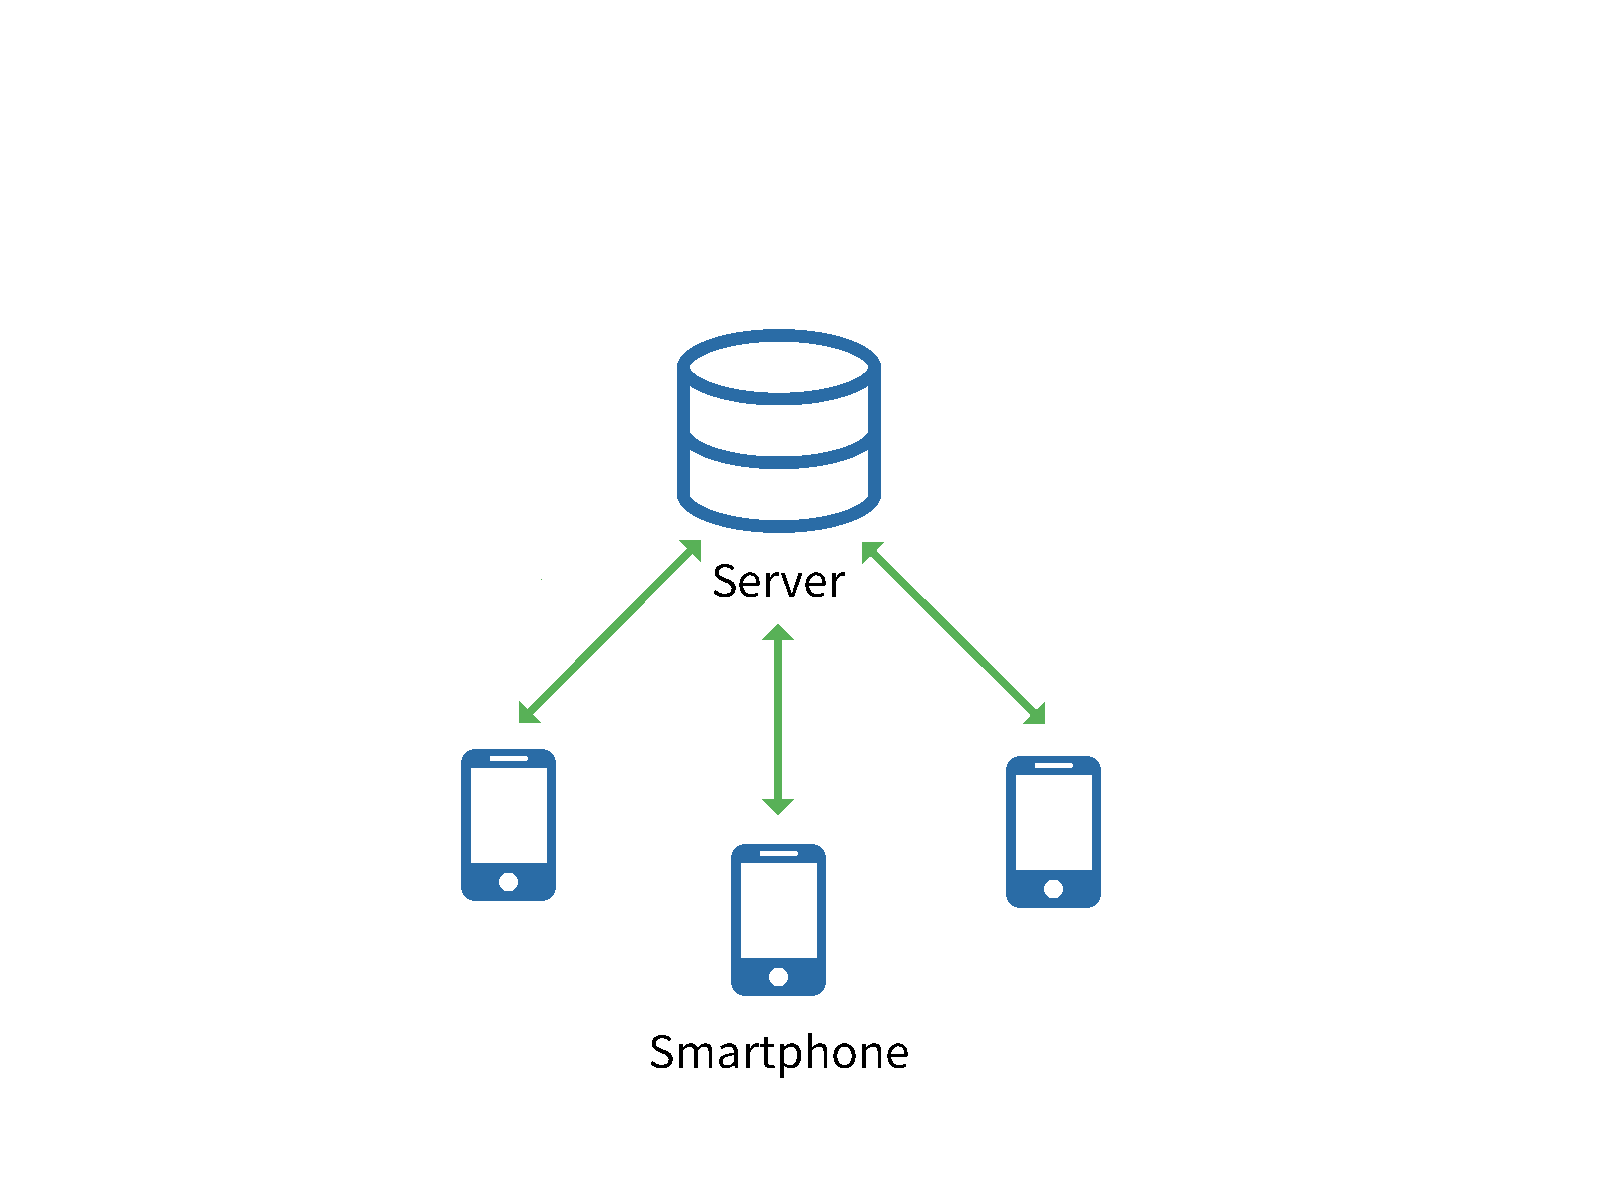
\includegraphics[height=6cm]{logos/client-server.png}
	\caption{Our client-server model}
	\label{img:client-server}
\end{figure}
The system is implemented according to the client-server model (figure \ref{img:client-server}). Users utilize a smartphone as a client, while the operator provides a server on which a central database is hosted. Also running on the server is a web service that can be requested by the clients via a REST API. The web service forwards the request to the database system and also returns the response back to the clients. An Android prototype was developed for the clients using Java. The web service is also written in Java and runs on a Tomcat server, while a MySQL server has been set up for the database system. In total, the implementation consists of three relatively independent parts, which will be examined in more detail below. The final realization of the $SPS$ is of course not part of this work or the implementation, but the last part of this section should give some comments on a possible realization. These include, for example, how to deal with the problem described at the end of section \ref{sec:Adversary Model and Assumptions} of adversaries not registered in the system.

\begin{figure}
	\centering
	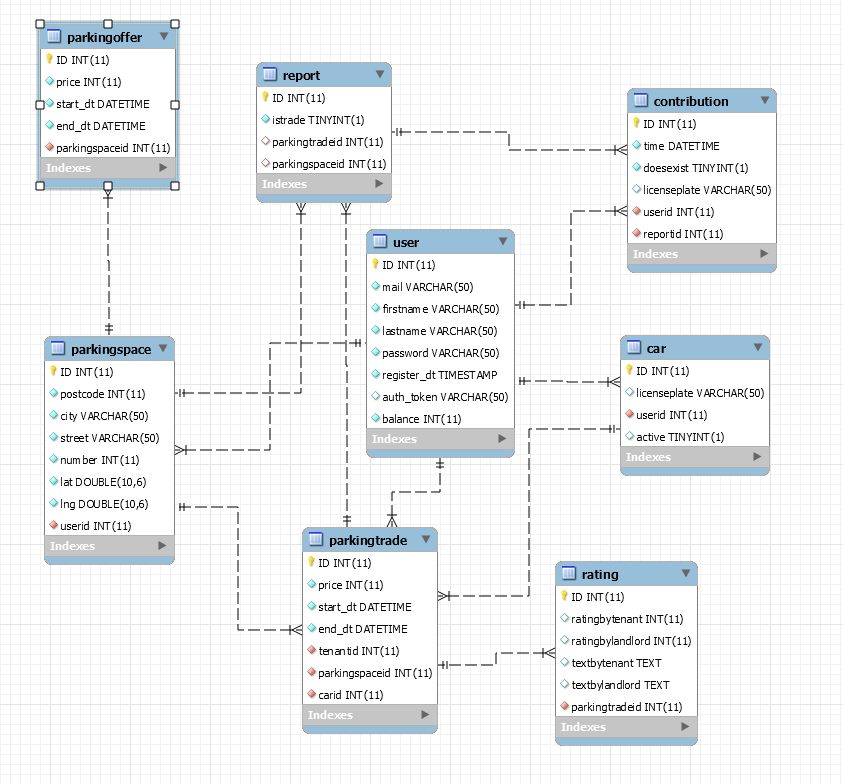
\includegraphics[width=14cm]{logos/eer-diagramm.png}
	\caption{The EER Diagramm of the database}
	\label{img:eer-diagramm}
\end{figure}

\section{Database}
A relational database management system was used to store user and parking data. We chose the open source system MySQL, which, as the name suggests, uses SQL as the query language. The actual database system, whose EER diagram is depicted in figure \ref{img:eer-diagramm}, consists of the following tables:
\begin{itemize}
\item \textbf{user:} Table \textit{user} represents a user $u \in U$ and stores attributes like mail, name, encrypted password, balance or reputation score.
\item \textbf{parkingspace:} Table \textit{parkingspace} represents a parking space $p \in P$ registered by a user and stores attributes like the address, coordinates and references the \textit{user}, who registered the parking space, with a foreign key constraint.
\item \textbf{parkingoffer:} Table \textit{parkingoffer} represents a parking offer created by a user for one of his parking spaces and stores attributes like offer starting time, offer ending time, price per hour and references the \textit{parkingspace}, for which the  offer was created for, with a foreign key constraint and thus allows to also figure out the user that created it.
\item \textbf{car:} Table \textit{car} represents a car registered by a user and stores the license plate, whether or not it is the active car of the user and references the \textit{user}, who registered the car, with a foreign key constraint. Every user can have a maximum of one car active at a time. If a user books a parking space this car is referenced in the \textit{parkingtrade} table.
\item \textbf{parkingtrade:} Table \textit{parkingtrade} represents a parking trade or contract between two users and stores attributes like booked starting time, booked ending time, price per hour and references the tenant \textit{user} and his \textit{car} as well as the \textit{parkingspace}, that was booked, with foreign key constraints and thus allows to also figure out the landlord that owns the parking space.
\item \textbf{rating:} Table \textit{rating} represents a rating for a parking trade and stores the rating value and text by both the landlord and the tenant of the parking trade and references the \textit{parkingtrade}, for which this rating was issued, with a foreign key constraint.
\item \textbf{report:} Table \textit{report} represents a report for a parking trade or parking space and stores for which one of the two the report is issued and references the \textit{parkingtrade} or \textit{parkingspace}, for which this report is issued, and the reported and reporting \textit{user}s with foreign key constraints.
\item \textbf{contribution:} Table \textit{contribution} represents a contribution to a report and stores the inspection time, whether the reported parking place exists, the license plate of the car parked on it at inspection time and references the \textit{user}, who gave the contribution, and the \textit{report}, for which this contribution applies, with foreign key constraints.
\end{itemize}

\subparagraph{Instructions for use}
To avoid having to recreate the database, a dump \textit{shared\_parking\_dump.sql} has been created that can be used to restore the database. This back up is located on the attached CD in the directory 'database'.

\section{Java Web Service}
A web service in Java was developed to access the database. It runs on a Tomcat server and offers a RESTful interface. This interface is used by the android app to access the database. The java open source framework Jersey is used to develop the REST API. This framework helps to address JAX-RS, the Java API for RESTful Web Service. For this purpose, annotations are used in the code that can be found in the java package javax.ws.rs. These annotations are used to specify the path and the request method, which are both part of an http request, by which a java method may be addressed.\\

The java code for the web service can be found on the attached CD in the directory 'web\_service'. The .java classes can be found in \textit{shared\_parking/src/com/shared\_parking}.

The package \textit{jersey} contains classes for every database table, in which the already addressed annotations are used to tell jersey for which HTTP request to listen. In these classes the web service functions are described. Those get called when the Tomcat server receives an appropriate HTTP request. For most of the tables the basic functions of persistent storage \textit{create, read, update and delete (CRUD)} are implemented. For some tables there are multiple \textit{read} functions, depending on how they are required by the android prototype. Car.java for example has two read methods: one for reading all cars by a user, another one for reading only the active car by a user. The data transferred between these web service functions and the android app is always in the form of JSON objects. Each of those functions receives their parameters as a JSON object in the body of the HTTP request and returns the result as a JSON object in the body of the HTTP response. The JAX-RS annotations used for all of our functions tell those function to listen to HTPP POST requests with MediaType.APPLICATION\_JSON as input and return value. After receiving a request, these web service functions then deconstruct the JSON Object into the represented parameters and calls another method, which then accesses the database.

The methods used for Database access can be found in the package \textit{dbconnection}. There is a database connection method for every web service function. The database connection methods take the deconstructed JSON object as parameters. They then open a database connection with the help of the java.sql package and create and execute the appropriate SQL querys. After receiving the Resultset from the database they call a utility method to create a JSONObject as the result and return it to the web service methods, which they then put into the HTTP response.

The utility methods can be found in the \textit{utility} package. They accept a java.sql Resultset and construct a JSON object from it, which they then return back to the database connection methods. 

\subparagraph{Instructions for use}
There is a class called Constants.java in the \textit{dbconntection} package. In there one has to change the parameters for database access, so that they match with the access information of ones own database. The whole project can for example be imported into Eclipse and the web service methods can be run in there on a Tomcat server.

\section{Java Android Prototype}
The main part of the implementation was the development of the android app, which is also written with java. The app uses Gradle as a build automation system. The development of the UI largely adheres to the guidelines set by Google regarding material design. This ensures that new users can find their way around the app in no time. The app itself has no internal database and mainly uses JSON objects to manage the user and parking data, since the data is returned in this form by the Web service. These objects are only stored in the random access memory and the corresponding web service is queried again if necessary.

For remembering a user session an auth\_token is stored in the Android Shared Preferences. This prevents the user from having to constantly enter his password. Despite that, the other information security features mentioned in the beginning of section \ref{Security Requirements}, like the encrypted network traffic, are not implemented as this is still a prototype used for testing.

The prototype implements all functional design features. Instead of giving the user the ability to charge and withdraw money, buttons are added which allow to adjust the balance of a user. Of the security design features, only the report module is implemented in the prototype. The other features are not necessary for an initial function test and only become meaningful when a test run is started with several users.

The java code for the prototype can be found on the attached CD in the directory 'android'. All the Gradle files can be directly found in this directory and in the subdirectories '.gradle' and 'gradle'. The .java classes can be found in \textit{app\-/main\-/ja\-va\-/com\-/e\-xam\-ple\-/sha\-red\-\_par\-king\-/src\-/com\-/sha\-red\-\_par\-king}. The .xml layout and menu files and the icons used for the UI can be found in \textit{app/main/res} in the corresponding subdirectories. The .java classes are divided into the package \textit{activities}, which contains all the code for the android activities and fragments and the package \textit{networking}, which contains all the code needed for getting access to the database through the web service functions by sending HTTP requests.

The class NetworkUtilities.java in the \textit{networking} package contains a static method for every CRUD web service function available. Those methods first construct the JSON object added into the body of the http request and then use the HTTP library Volley to send a HTTP request. The JSON object that is returned by the web service can processed through the implementation of a callback interface called ServerCallback.java.

The \textit{activities} package is further divided. First, there is the BaseActivity.java which defines the Toolbar and the DrawerLayout with integrated NavigationView. Every other activity class extends this BaseActivity, thus enabling the toolbar and the drawer menu at all times. Each menu item in this drawer menu (figure \ref{img:screenshot-menu}) has its own subpackage containing the corresponding activity and all corresponding fragments. The following menu items and packages exist:

\begin{itemize}
\item \textbf{Home:} The java classes for the 'Home' menu item are found in the \textit{main} package. The package contains the MainActivity and two fragments, which provide the ability for the user to log in and register.
\item \textbf{Search for parking:} The java classes for the 'Search for parking' menu item are found in the \textit{search} package. The package contains the SearchActivity, which displays a SupportMapFragment, and two DialogFragments. The SupportMapFragment shows a map provided by Google, on which the available parking spaces are displayed as markers (figure \ref{img:screenshot-search}). The DialogFragments serve on the one hand to select the date and time at which a parking space should be searched for (TimeDialogFragment), on the other hand to display information about this parking space with the possibility of confirming the booking (ParkingOfferDialogFragment).
\item \textbf{Contracts:} The java classes for the 'Contracts' menu item are found in the \textit{contracts} package. The ContractsActivity uses a TabLayout to create tabs and divide the parking contracts into contracts as landlord and contracts as tenant. There is a fragment for both tabs, which contains a RecyclerView that utilizes the ContractsAdapter. A RecyclerView is a layout element that allows to create scrollable list of objects which are defined in an adapter. Here all the parking contracts of the user with further information are displayed.
\item \textbf{My Offers:} The java classes for the 'My Offers' menu item are found in the \textit{parkingoffer} package. In this case OffersListFragment provides a RecyclerView with OffersAdapter. In addition, there is a OffersAddFragment that allows you to add and edit parking offers.
\item \textbf{My Parking Spots:} The java classes for the 'My Parking Spots' menu item are found in the \textit{parkingspots} package. This package contains the same classes and functionality as the \textit{parkingoffer} package. It shows a list of the users parking spaces and allows him to add new ones, edit or delete existing ones.
\item \textbf{My Profile:} The java classes for the 'My Profile' menu item are found in the \textit{profile} package. The ProfileActivity uses a TabLayout to create tabs and divide the profile view into general profile and cars. The ProfileGeneralFragment show general information about the user, such as mail, name and balance and allows the user to adjust the balance. The CarListFragment works in the same way as the other list fragments and provides a list of the users' cars.
\item \textbf{Report a violation:} The java classes for the 'Report a violation' menu item are found in the \textit{report} package. There is a ReportFragment which allows users to report adversaries either at a parking contract or parking place.
\item \textbf{Logout:} There are no java classes and no package for the 'Logout' menu item. Clicking on this menu item simply disconnects the user by deleting the saved auth\_token.
\end{itemize}

\begin{figure}
	\centering
	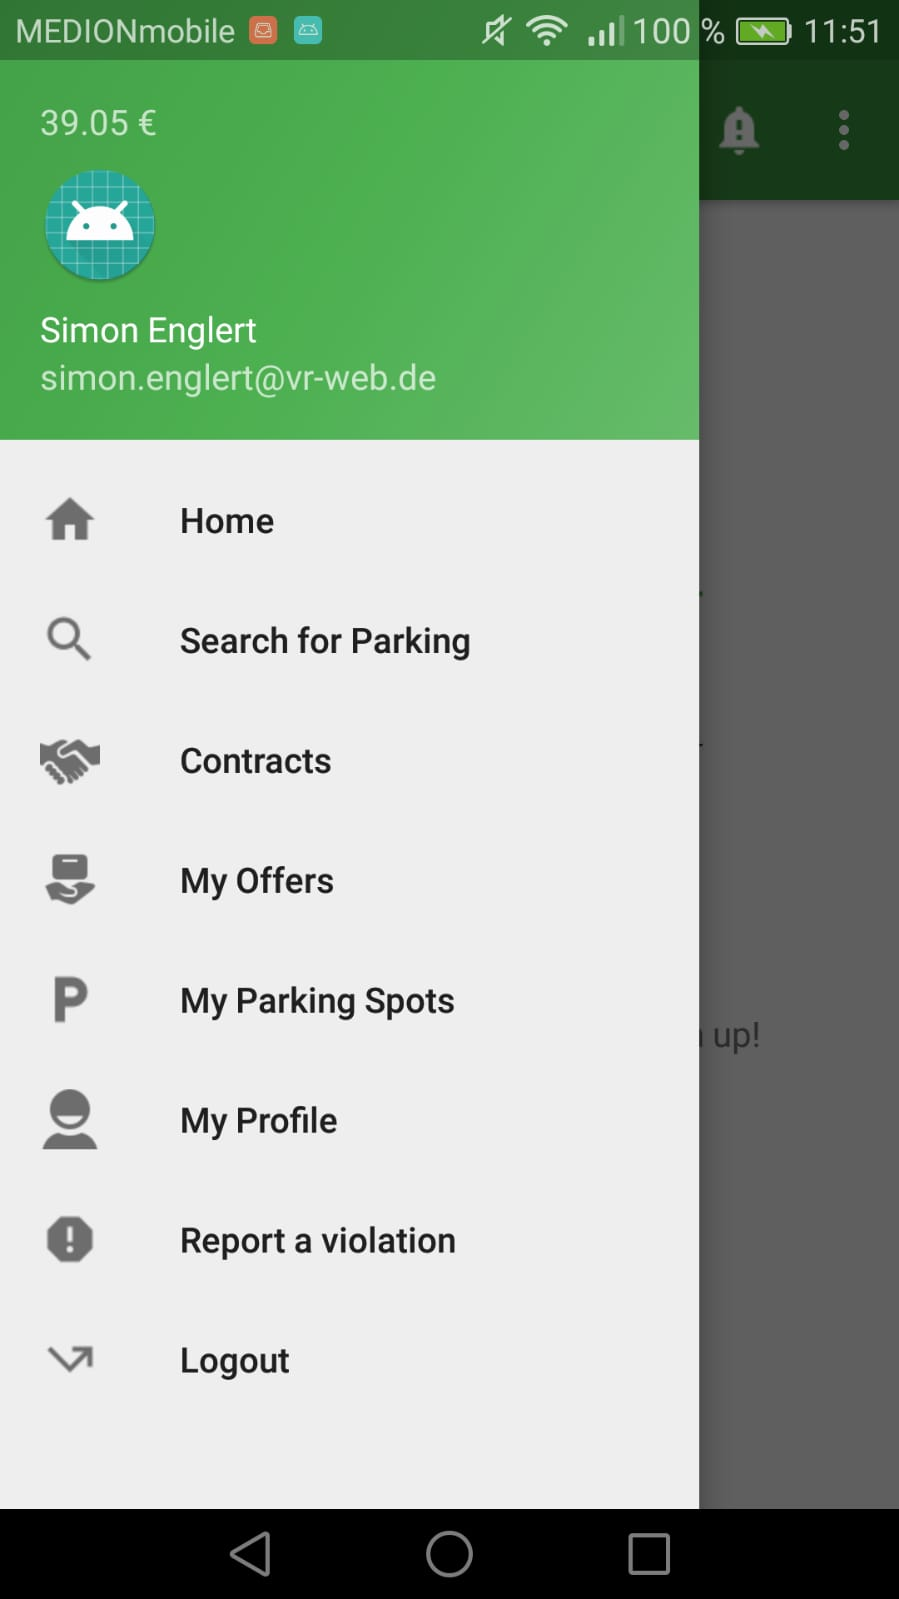
\includegraphics[height=11cm]{logos/screenshot-menu.png}
	\caption{A screenshot of the drawer menu of the prototype}
	\label{img:screenshot-menu}
\end{figure}

\begin{figure}
	\centering
	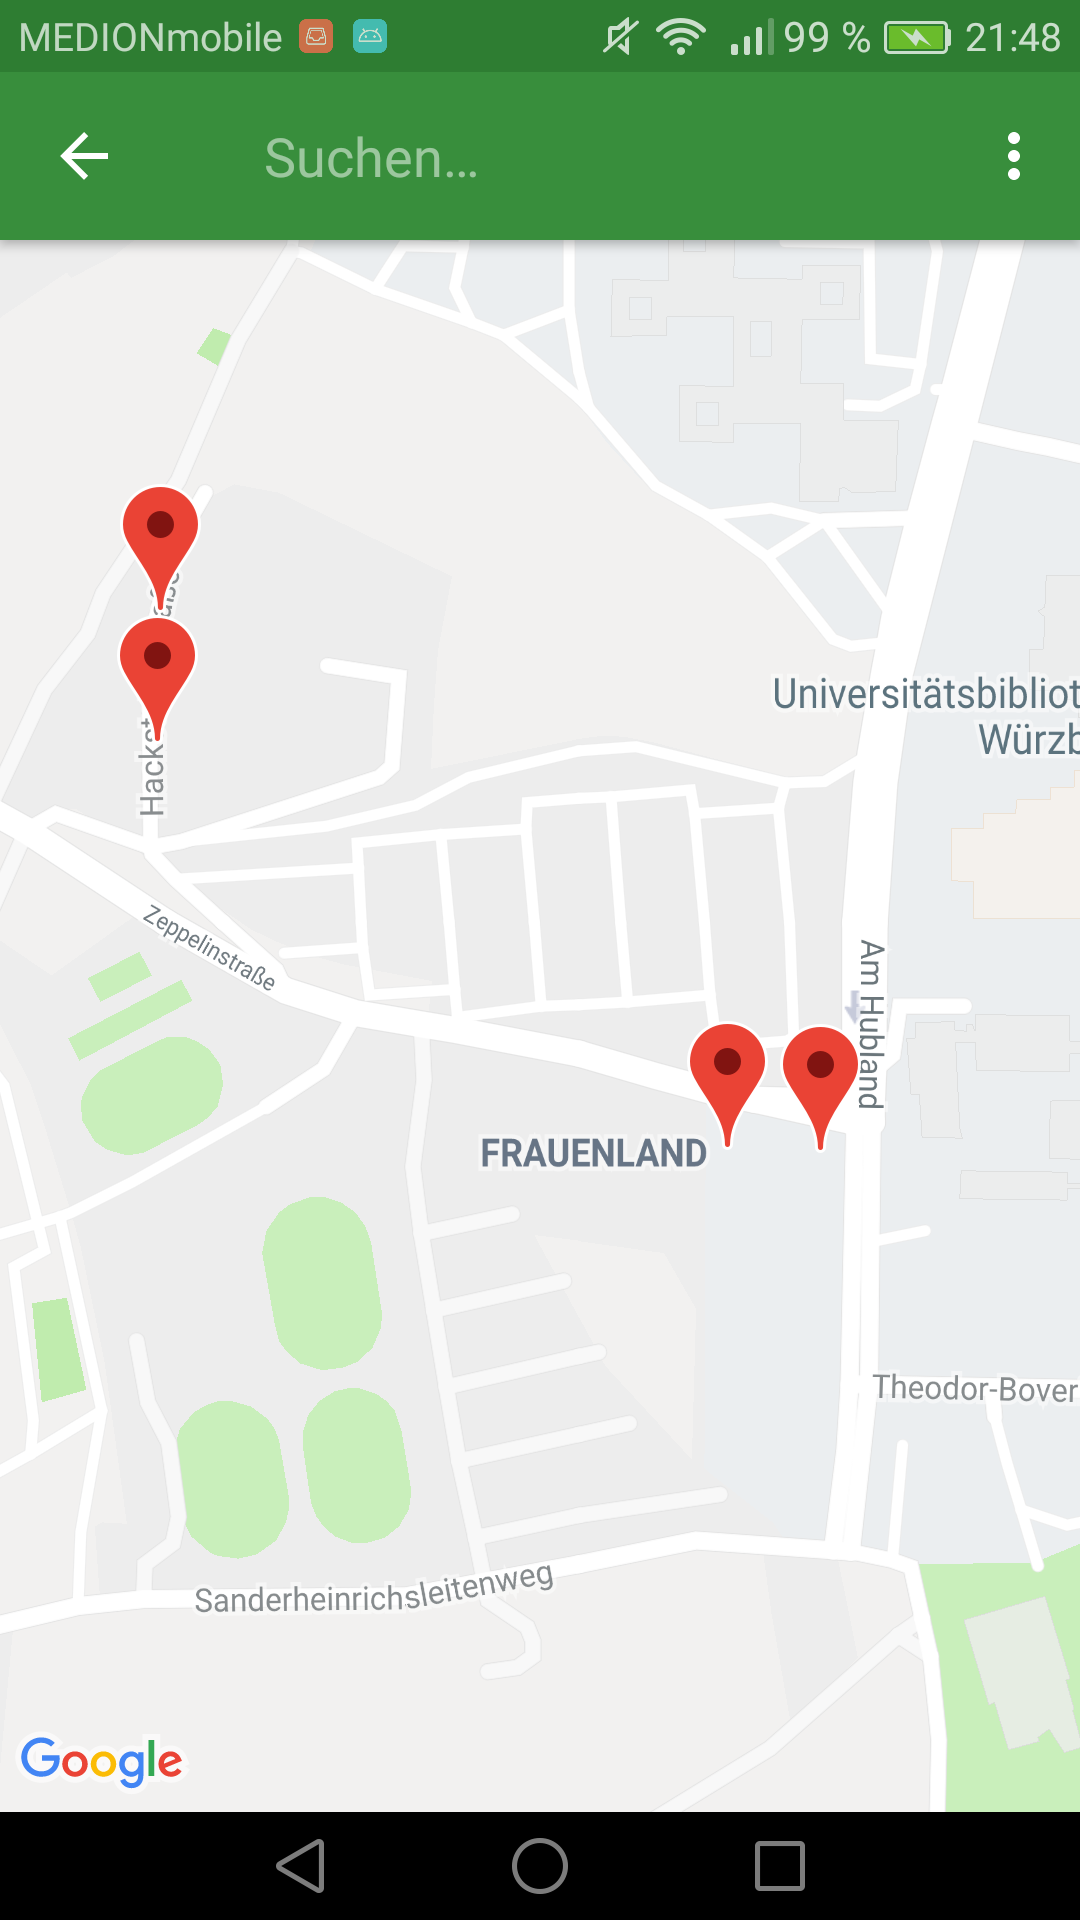
\includegraphics[height=11cm]{logos/screenshot-search.png}
	\caption{A screenshot of the parkingplace search feature of the prototype}
	\label{img:screenshot-search}
\end{figure}

\subparagraph{Instructions for use}
One has to adjust the static String BASE\_URL found in line 21 of NetworkUtilities.java in the package networking to the server address of the Java web service. The whole project can for example be imported into Android Studio and the app can be run on a connected android smartphone or an emulated device in Android Studio.

\section{Comments on the realization of the $SPS$}\label{sec:Comments on the realization}

\subparagraph{Creation of a basic user structure}
The problem of many shared parking systems mentioned in section x is that they could hardly generate any users at all. One of the reasons for this is probably that such a system must first overcome a certain barrier before it becomes attractive for users. Nobody registers with a system to lease parking spaces if there is no one renting them out. And no private user takes the trouble to insert a parking space that nobody will ever book. The pure C2C model is actually not really suited for the launch of such a system. However, businesses can help to overcome this barrier. Various buisenesses such as hotels, cinemas, doctors or supermarkets usually only need their parking spaces for a certain period of the day. If one has already contacted some of the above mentioned before launching the system and they decide to insert their parking spaces, the system already launches with a large supply of parking spaces. This supply can then also ensure that demand increases and the system further grows.

\subparagraph{Solution for adversaries not registered in the system}
In section x the problem has already been raised that it is not possible to punish parking offenders directly via the $SPS$ if they are not part of the system. However, there is also a solution that can be implemented when realizing the system.

Without the $SPS$, adversaries in private parking spaces can only be punished by requesting a towing service and having the parking space cleared. There are, however, two problems: On the one hand, all costs that the adversary has to pay are transferred to the towing service and cannot be used by the $SPS$ to pay for a replacement parking space or inspectors. On the other hand, it can happen that the adversary has already left the parking space when the towing service arrives and the caller has to cover the costs.

However, the situation that several towing services are competing with each other in larger cities can be taken advantage of. It should be possible to negotiate a deal with one of the towing services stating that all towing operations under the $SPS$ will be carried out by this service provider. In return, the service provider pays part of its extremely high towing fee back to the $SPS$, which can then be used to pay for the replacement parking space and the inspectors. In addition, service provider should not charge any costs in the event that the adversary has already left the car park. In return, every report, that contains a license plate which is not registered in the system, is forwarded directly to the towing service. In this way, both parties can benefit from the deal.
\chapter{Future Work}
\label{ch:Future Work}
To conclude, we will present some further aspects of this topic which either could not be elaborated within the time frame of the study or which would exceed the scope of this work. These can be carried out in further work.

\subparagraph{Using Trusted Platform Modules as Trust System for the $SPS$}
In section \ref{sec:Trust Systems} two methods for implementing a trust system were presented. On the one hand, there is a trust system based on a reputation score, as implemented in this work. On the other hand, trusted platform modules can be used to check whether users have tampered with their contributions. In further work, TPMs could be used to ensure that a report is valid. This could save the use and payment of inspectors.
\subparagraph{Extending the functionality of the app}
The app should be extended in the future. On the one hand, not all the security functions presented in this paper have been implemented. On the other hand, there are opportunities to set up convenience functions in many places.
\subparagraph{Testing the usability of the app}
One objective of the app should be good usability, which means the implementation of the basic features and use cases should be intuitive to use. First time users should be able to book or rent out a parking space in a few clicks. We believe that we have reached this goal, but to prove it a user study would have to be prepared and conducted. This could done as a part of a follow-up work.
\subparagraph{Testing the performance of the app}
The same applies to performance. Our app should show consistently good performance, preventing annoying waiting or loading times for the user. The verification of the performance could also be carried out in a user study.
\subparagraph{Proving the profitability of the $SPS$}
If a service provider wanted to realize the $SPS$, it should be verified beforehand that the system will in total generate profits and not losses. Although the $SPS$ was developed with this property in mind, test models and calculations would have to be carried out to check its profitability. Such models and calculations are outside the scope of an computer science bachelor thesis like this one, but can be carried out in future work.

\chapter{Conclusion}
\label{ch:Conclusion}
In conclusion, it can be noted that a shared parking system has been developed in this work that allows users to rent and let parking spaces, which in particular can successfully deal with a series of attacks. This distinguishes the $SPS$ from state-of-the-art shared parking systems. The functionality of the $SPS$, especially the protection against fraud, the punishment of adversaries, and the compensation of injured parties works without significant deployment costs and largely without manual intervention by the $SP$. The android prototype developed as part of this study reflects the basic functions and shows good usability and performance in first tests. Finally, topics for further research were provided.
\chapter{Acknowledgments}
\label{ch:Acknowledgments}
I would like to thank Prof. Dr. Alexandra Dmitrienko and the city of Würzburg, who both supported me in creating this thesis.



%% ----------------
%% |   Appendix   |
%% ----------------
%%\cleardoublepage

%%\printnoidxglossaries

%%\cleardoublepage

%%\appendix

\iflanguage{english}
{\addchap{Appendix}}	% english style
{\addchap{Anhang}}	% german style
		
\setcounter{figure}{0}

\section{A}



%% --------------------
%% |   Bibliography   |
%% --------------------
\cleardoublepage
\phantomsection
\addcontentsline{toc}{chapter}{\bibname}

%\iflanguage{english}
%{\bibliographystyle{IEEEtranSA}}	% english style
%{\bibliographystyle{babalpha-fl}}	% german style

%\bibliographystyle{plainnat}
												  
% Use IEEEtran for numeric references
\bibliographystyle{IEEEtranSA}

\bibliography{thesis}

\end{large}
\end{document}